%======================================================================
%   Zak Webb
%   Ph. D. Thesis
%   Department of Physics and Astronomy
%   University of Waterloo
% 
%   Scattering on Graphs
%======================================================================


\documentclass[../thesis-main/thesis-main]{subfiles}
\begin{document}

\chapter{Scattering on graphs}
\label{chap:scattering_on_graphs}


Since scattering is useful as an analytic tool near everywhere in physics \cite{RSScat}, one might at the usefulness of scattering in quantum information.  High energy physics uses scattering to probe atoms and molecules, but we would want to discretize the system for use in quantum information.  In this manner, we would replace the continuum by a discrete set of positions, and understand the evolution in such a model.

With this discretization, we are analyzing a system propagating on an infinite graph, and thus we can also think of this as the limit of a continuous time quantum walk to infinite graphs.  We know that quantum walks are useful algorithmic devices (e.g., \cite{CCDFGS03,Amb07}), and one might wonder whether these infinite systems can allow for intuitive algorithms.  It turns out that this answer is yes, and the original motivation for graph scattering was an algorithm using graph scattering to solve a problem for decision trees \cite{FG98}, which eventually led to an algorithm solving boolean formulas faster than any randomized classical computation \cite{FGG08}.  This algorithm was easily understood using the intuition from scattering, and thus graph scattering became a useful tool for understanding quantum walk algorithms.

This chapter should serve as a broad introduction to graph scattering.  In particular, the notations of scattering matrices, bound states, and wave-packets have all been used in previous works.  This chapter attempts to standardize notations, while also explaining how everything works.  While there is some original work in this chapter, we also utilize and state several of the results from \cite{FGG08,Chi09,CS11,CG12} in which the author did not contribute.

\section{Free particles in the continuum}

Let us first take a look at one of the most simple quantum systems seen in any quantum mechanics text (e.g., \cite{GriQM} or \cite{SakMQM}): a free particle in one dimension.  Without any potential or interactions, we have that the time independent Schr\"{o}dinger equation reads
\begin{equation}
  \frac{\partial^2}{\partial x^2} \psi(x) = -\frac{2m}{\hbar^2}E \psi(x) = -k^2 \psi(x),
\end{equation}
which requires the (unnormalizable) solutions,
\begin{equation}
  \psi(x) = A \exp(- i k x) + B \exp(i k x) \label{eq:simple_motivating_momentum_states}
\end{equation}
for real $k$ and for arbitrary constant $A$ and $B$.  These \textit{momentum states} correspond to particles travelling with momentum $k$ along the real line, and they span the Hilbert space.  Note that these momentum states are not technically within the Hilbert space, since they are not normalizable. 

While these momentum states are useful for understanding the propagation of particles in the quantum setting, if we want to understand more complicated behavior we need to change the potential energy of the system.  In particular, we will now include some finite-range potential $V$ that is non-zero only for $|x| < d$ for some constant $d$, so that outside this range the eigenstates remain unchanged.  The only difference is that we will deal with a superposition of states for each energy instead of the pure momentum states, forcing some relation between the $A$ and $B$ of equation \eq{simple_motivating_momentum_states}.  Namely, the eigenstates of this system become
\begin{equation}
  \psi(x) = \begin{cases}
    \exp(-i k x) + R(k) \exp(i k x) & x \leq -d\\
    T(k) \exp(- i k x) & x \geq d\\
    \phi(x,k) & |x| \leq d
    \end{cases}
\end{equation}
for some functions $R(k)$, $T(k)$, and $\phi(x,k)$ that depends on the interaction $V$.  As intuition, these states can be seen as a particle with momentum $k$ coming in from the left, hitting the potential, and then scattering (which motivates the $T$ and $R$ labels).  

In addition to these scattering states, it is also possible for bound states to exist.  These are normalizable states that have a constant fraction  of their amplitude near the non-zero potential, so that they do not affect scattering states that originate far from the interaction.  They simply exist as additional states in the Hilbert space.


\subsection{Free particles on an infinite path}

With the simple free-particle example in mind, let us now examine the discretized system.  Namely, instead of allowing arbitrary real positions, let us restrict attention to some regular 1-D lattice, such as the natural numbers.  Further, much as there is a natural linear ordering on the positions in the continuum, and in order for a particle to move between $a$ and $b$ it must travel over all positions between $a$ and $b$, in the discretized system we only allow particles to move between adjacent integers.  Explicitly, the position basis for this discretized Hilbert space will be labeled by $n\in \NN$, with transport only allowed between integers that differ by one.

If we then want to understand how this discretized system works, it will be useful to discretize the entire Schr\"{o}dinger equation.  Along those lines, remember that the second derivative of a function $f$ at $x$ can be written as
\begin{align}
  \frac{d^2}{dx^2} f(x) = \lim_{h\rightarrow 0} \frac{f(x+h) - 2 f(x) - f(x-h)}{h^2}.
\end{align}
Since we were originally working in the continuum, we could let $h$ go to zero without any problems.  In our discretize world, however, there exists some smallest difference in $x$, namely 1.  As such, we have that in our discretized space, the operator corresponding to the second position derivative can be written as
\begin{equation}
  \Delta^2 = \sum_{x=-\infty}^\infty \ket{x} \big(\bra{x-1} - 2 \bra{x} + \bra{x+1}\big) = \sum_{x=-\infty}^\infty \big(\ketbra{x}{x-1} + \ketbra{x}{x+1}\big) - 2 \II.
\label{eq:discrete_second_derivative}
\end{equation}
If we then rescale the energy levels, we have that the identity term in the right hand side of \eq{discrete_second_derivative} can be removed, so that $\Delta^2$ on this discretized one-dimensional system is proportional to the adjacency matrix of an infinite path.  

With this representation of the second derivative operator, we can see that when discretized, the time-independent Schr\"{o}dinger equation for a free particle becomes
\begin{equation}
  \Delta^2 \ket{\psi} = \Big(\sum_{x=-\infty}^\infty \big(\ketbra{x+1}{x} + \ketbra{x-1}{x}\big) - 2 \II\Big) \ket{\psi} = E'_{\psi} \ket{\psi}.
\end{equation}
If we rescale the energy term, and then break the vector equation into its components, we find that
\begin{equation}
  \braket{x+1}{\psi} + \braket{x-1}{\psi} = E_\psi \braket{x}{\psi}
\end{equation}
for all $x\in \ZZ$.  Taking motivation from the continuous case,  we then make the ansatz that $\braket{x}{\psi} = e^{i k x}$ for some $k$, and find
\begin{align}
  \braket{x+1}{\psi} + \braket{x-1}{\psi} = e^{i k } e^{i k x} + e^{-ik} e^{ikx} &= E_\psi e^{ik x} = E_\psi \braket{x}{\psi}  \\ E_\psi &= e^{ik} + e^{-i k} = 2 \cos(k).
\end{align}
If we then use the fact that $E_\psi$ must be real, and that the amplitudes should not diverge to infinity as $x\rightarrow \pm \infty$, we find that the only possible values of $k$ are between $[-\pi,\pi)$.    Hence, in analogy with the continuous case, the eigenbasis of the Hamiltonian corresponds to momentum states, but where the possible momenta only range over $[-\pi,\pi)$.  We represent this momentum state with momenta $k$ as $\ket{\tilde{k}}$.  Note that similar to the continuum, these momentum states are not technically in the relevant Hilbert space.  This won't won't be problematic for our purposes, but it can lead to some headaches

Additionally, we can discuss the ``speed'' of these eigenstates, which is given by the derivative of the energy with respect to momentum.  We con then see that 
\begin{equation}
  s = \Big| \frac{d E_k}{d k} \Big| = 2 \sin (|k|),
\end{equation}
which is to be compared with $s \propto |k|$ for in the continuum case.  While the discretization does change the relationship between momentum, energy, and speed, if we restrict ourselves to small $k$ (so that the discretization is not noticeable), we recover the linear relationship.  In this way, as the distance between vertices grows smaller, we recover the continuum case.  

One problem that is unique to our discretized system is that  there are an uncountable number of momentum states, while the position basis contains only a countable number of basis states.  It turns out that the resolution to this conundrum is that the two bases have different orthogonality conditions: the position basis elements are Kronecker delta orthogonal, while the momentum basis elements are Dirac $\delta$-function orthogonal.  Namely,
\begin{equation}
  \braket{\tilde{k}}{\tilde{p}} = \sum_{x=-\infty}^\infty e^{- i k x} e^{i k p} = \sum_{x=-\infty}^\infty e^{i (p-k) x} = 2\pi \delta(p-k),
\end{equation}
so that we can decompose the identity on this space as 
\begin{equation}
\II = \sum_{x=-\infty}^\infty \ketbra{x}{x} = \frac{1}{2\pi} \int_{-\pi}^\pi dk \ketbra{\tilde{k}}{\tilde{k}}.
\end{equation}


%%%%%%%%%%%%%%%%%%%%%%%%%%%%%%%%%%%%%%%%%%%%%%%
\section{Graph scattering}

Essentially, at this point we have recovered many of the results of the continuous free particle, but with a discretized position space.  The main idea behind the discretization was the change in the second derivative operator, and noting that it became proportional to the adjacency matrix of a simple graph.  This seems very similar to the case of continuous time quantum walks, in which the Hamiltonian is explicitly taken to be the adjacency matrix of a (finite sized) graph. 

As such, let us assume that the Hamiltonian of the entire system is proportional to the adjacency matrix for these graph scattering problems.  If we now want to add some finite potential to the system, in an attempt to discretize the scattering formalism, we could add a potential function, with explicit potential energies at various vertices of the infinite path.  However, if we wish to examine scattering only on unweighted graphs, we need to be a little more clever.  

To solve this problem, we will connect graphs in such a way that far from our connections the graphs will look identical to that of an infinite path, but near our changes the graph can differ drastically from an infinite path.  In particular, we will use an arbitrary (finite) graph as a base, and connect semi-infinite (infinite in one direction) paths to this base graph.

With this construction, the eigenvalue equation must still be satisfied along the semi-infinite paths, and thus the form of the eigenstates along the paths must still be of the form $e^{i k x}$ for some $k$ and $x$.  However, we can no longer assume that $k$ is real, as the fact that the attached semi-infinite paths are only infinite in one direction allow for an exponentially decaying amplitudes along the paths.  Additionally, we can have nontrivial correlations between the amplitudes among the different paths, similar to the correlated reflection and transmission coefficients in the continuous case.

Note that the topic of graph scattering has appeared previously in the literature.  Most of this section is not original work, and should be taken as background material.  In particular, these results are taken from \cite{FGG08, Chi09, CS11, CG12}.  I will also include 


%%%%%%%%%%%%%%%%%%%%%%%%%%%%%%%%%%%%%%%%%%%%%%%
\subsection{Infinite path and a Graph}\label{sec:infinite_path_and_graph}

In the most simple example, let us attached a graph $\widetilde{G}$ to an infinite path.  In particular, we assume that $\widetilde{G}$ is attached to a single vertex of the infinite path, and that the graph is attached by adding an edge from each vertex in $S\subset V(\widetilde{G})$ to one specific vertex of the infinite path, which we label $0$, as seen in \fig{path_and_graph}.  Calling this new graph $G$, the adjacency matrix of $G$, and thus the Hamiltonian for this scattering problem, can be seen to be
\begin{equation}
  A(G) = A(\widetilde{G}) + \sum_{v\in S \subset V(\widetilde{G})} \ketbra{v}{0} + \ketbra{0}{v} + \sum_{x=-\infty}^\infty \ketbra{x}{x+1} + \ketbra{x+1}{x}.
\end{equation}

If we then want to inspect the eigenvectors of this Hamiltonian, we find that the eigenvalue equation remains unchanged for non-zero vertices on the path.  Hence, we can see that any eigenstate of the Hamiltonian must take the form $Ae^{i k x} + Be^{-i k x}$ for some $k$ along the infinite paths.  


%%%%%%%%
\begin{figure}
  \centering
  \tikzsetnextfilename{GS_path_and_graph}
  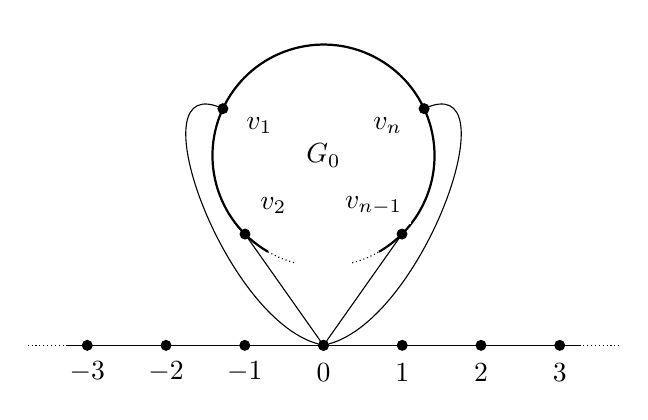
\begin{tikzpicture}[
  label distance=-5.5pt,
  thin,
  vertex/.style={circle,draw=black,fill=black,inner sep=1.25pt,
    minimum size =0mm},
  attach/.style={circle,draw=black,fill=white,inner sep=1.25pt,
    minimum size =0mm},
  dots/.style={circle,fill=black,inner sep=.5pt,
    minimum size= 0pt}]

% Path and Labels    
  \draw (-3.25,-2.41) -- (3.25,-2.41);
  
  \foreach \x in {-3,...,3}{
    \node at (\x,-2.41) [vertex] {};
    \node at (\x,-2.75) {$\x$};
  }
    
  \node (a) at (0,-2.41) [vertex] {};
  
  \draw[densely dotted] (-3.25,-2.41) -- (-3.75, -2.41);
  \draw[densely dotted] (3.25, -2.41) -- (3.75, -2.41);
  
% Graph  
  \draw[thick] (240:1.41) arc (240:-60:1.41);
  \draw[densely dotted] (240:1.41)  arc (240:255:1.41);
  \draw[densely dotted] (285:1.41)  arc (285:300:1.41);
  
  \foreach \i / \n /\t in {25 / n/ 15, 155 / 1/ 165, 225/ 2 / 120, 315 / {n-1}/60}{
    \node at (\i : .9) [rectangle,fill=white] {$v_\n$};
    \node at (\i : 1.41) [vertex] {};
  }
  \node at (0,0) [rectangle,fill=white] {$G_0$};

% Attaching Edges
  \foreach \i /\t in {25/15, 155/165}{
    \draw (\i:1.41) to[out=\i,in=\t] (a);
  }
  
  \foreach \i \in in {225,315}{
    \draw (\i:1.41) to (a);
  }

\end{tikzpicture}
  \caption[Simple example for graph scattering]{A simple example for graph scattering.  A graph $\widetilde{G}$ is attached to an infinite path.}
  \label{fig:path_and_graph}
\end{figure}

With this assumption, we can see that there are three distinct cases for the form of the eigenstates.  In particular, the eigenstate could have no amplitude along the infinite paths, being confined to the finite graph $\widehat{G}$.  It could also be a normalizable state not confined to the finite graph $\widehat{G}$, in that the amplitude along the infinite paths decays exponentially.  Finally, the eigenstate could be an unnormalizable state, in which case we will call it a scattering state.

In the first case, where the state is confined to the graph $\widetilde{G}$, we have the major restriction that the state $\ket{\psi}$ satisfies 
\begin{align}
  \braket{x}{\psi} = 0
\end{align}
for all $x\in \NN$.  Additionally, if $\ket{\phi}$ is the restriction of $\ket{\phi}$ to the finite graph $\widetilde{G}$, we have that 
\begin{align}
  A(\widetilde{G}) \ket{\phi} = E \ket{\phi}
\end{align}
so that $\ket{\phi}$ is an eigenstate of the graph $\widetilde{G}$, that also satisfies
\begin{align}
  \sum_{v\in S} \braket{v}{\phi} = 0.
\end{align}
These restrictions together show that these completely bound states have an extremely restricted form as eigenstates of $A(\widetilde{G})$, but the infinite path does not really affect them.  In particular, their energies are not restricted by anything other than the graph itself, but we are guaranteed to have at most $|V(\widetilde{G})|$ of these confined bound states.

In the second case, we could have that the eigenstate is normalizable, but is not confined to the graph $\widetilde{G}$.  In this case, we have that the amplitudes along the infinite paths must go to zero, but they must still be a sum of exponentials.  As such, we have that $\ket{\psi}$ must be of the form
\begin{align}
  \braket{x}{\psi} = A z^x
\end{align} 
for some $z\in (-1,1)\setminus \{0\}$ for all $x\in \NN$, so that the energy must be $z+ z^{-1}$ (the case for $z= 0$ forces $A = 0$, and we are in the first case).  Additionally, we can see that if $\ket{\phi}$ is the restriction of $\ket{\psi}$ to those vertices inside the graph $A(\widetilde{G})$, they must satisfy
\begin{align}
  A(\widetilde{G}) + A \sum_{v\in S} \ket{v}\braket{v}{\phi} = 2 \cos (k) \ket{\phi},
\end{align}
a modified version of the eigenvalue equation for the graph $A(\widetilde{G})$.

Let us finally assume that the state is a scattering state.  Note that the eigenvalue of the state must be in the range $[-2,2]$, and that the form of the eigenstate along the paths must be scalar multiples of $e^{ikx}$ and $e^{-ikx}$, for some $k\in [-\pi, \pi]$.  Explicitly, the state must be of the form
\begin{align}
  \braket{x}{\psi} = \begin{cases} Ae^{i k x} + B e^{-i k x} & x \leq 0\\
   C e^{i k x} + D e^{-i k x} & x\geq 0\end{cases}
\end{align}
where the additional edges at $x=0$ can change the coefficients of each $e^{ik}$.  However, we do have that $A + B=C +D$, since the amplitude at $0$ is single valued, and that the eigenvalue of this state is given by $2\cos(k)$.  Note that we have not yet determined the form of the eigenstate inside the graph $\widetilde{G}$, but if we define $\ket{\phi}$ to be the restriction of $\ket{\psi}$ to the finite graph $\widetilde{G}$, then $\ket{\phi}$ must satisfy the equation
\begin{equation}
  A(G) \ket{\phi} + (A+ B)\sum_{v\in S} \ket{v}\braket{v}{\phi} = 2\cos(k) \ket{\phi},
\end{equation}
where the additional term arises from the fact that the vertices in $S$ are connected to the vertex $0$.  Finally, we have that
\begin{equation}
  2 \cos(k)\braket{0}{\psi} = Ae^{-ik} + B e^{ik} + C e^{i k} + D e^{-ik} + \sum_{v\in S} \braket{v}{\phi},
\end{equation}
since the eigenvalue equation must be satisfied at $0$.

In the first two cases, we have that the state is highly localized to the area surrounding the graph $\widetilde{G}$, and thus they do not have a large effect on wavefunctions that originate far from the graph.  However, the aptly named scattering states can be used to determine the time evolution of these wave functions.  In particular, if we look at the case where $A = 1$ and $D = 0$,  we can see that
\begin{align}
  \braket{x}{\psi} = \begin{cases} e^{-ikx} + B e^{i kx} & x\leq 0\\
  C e^{-ikx} & x \geq 0\end{cases}
\end{align}
so that $1+ B  =C$.  Note that this is reminiscent of a scattering state, with reflection amplitude $B$ and transmission amplitude $C$.  We can then take as intuition that these scattering states represent a wavepacket with momentum exactly $k$ traveling towards the graph $G$, and then scattering with these amplitudes.  We will use this intuition for our definitions of scattering on more general graphs. 
 
%%%%%%%%%%%%%%%
\subsection{General graphs}\label{sec:general_graphs}

Let us now turn our attention to scattering on more general graphs (and note that this section is very similar to \cite{CG12}).  In particular, let $\widehat{G}$ be any finite graph, with $N+m$ vertices and an adjacency matrix given by the block matrix
\begin{equation}
  A(\widehat{G}) = \begin{pmatrix}A & B^\dag\\ B & D\end{pmatrix},
\end{equation}
where $A$ is an $N\times N$ matrix, $B$ is an $m\times N$ matrix, and $D$ is an $m\times m$ matrix.  When examining graph scattering, we will be interested in the graph $G$ given by the graph-join of $\widehat{G}$ and $N$ semi-infinite paths, with an additional edge between each of the first $N$ vertices of $\widehat{G}$ and the first vertex of one semi-infinite path.  A schematic example can be seen in \fig{basic_graph}.

We shall label call the first $N$ vertices of the graph \emph{terminal vertices}, as they connect the semi-infinite paths to the finite graph $\widehat{G}$, and we shall label them as $(1,i)$, where $i\in[N]$.  Analogously, we will refer to the vertices on the $N$ semi-infinite paths as $(x,i)$ for $x\in \NN^+$ and $i\in[N]$, with the $i$ label referring to the particular semi-infinite path on which the vertex is labeled, while the label $x$ denotes the location along the path.  We also refer to the remaining $m$ vertices of $\widehat{G}$ as the \textit{internal vertices} of $\widehat{G}$, and label them as $w\in[m]$.  With this labeling of the vertices of $G$, the adjacency matrix of $G$ is then given by
\begin{equation}
  A(G) = A(\widehat{G}) + \sum_{j=1}^N \sum_{x=1}^\infty \big(\ketbra{x,j}{x+1,j} + \ketbra{x+1,j}{x,j}\big).
\end{equation}

At this point, we want to examine the possible eigenstates of the matrix $A(G)$.  It turns out that there are 3 different kinds of eigenstates, corresponding to the different qualitative properties of the eigenstate along the semi-infinite paths, exactly as in the case studied in \sec{infinite_path_and_graph}.

While we will mostly be interested in the third such type, corresponding to scattering off of the graph, the other two kinds remain important for a decomposition of the identity.  In particular, we will be guaranteed that these three kinds of eigenstates will form an orthogonal basis for the Hilbert space, and thus we will be able to use this decomposition to guarantee particular behavior of time evolved states.

\begin{figure}
  \centering
  \tikzsetnextfilename{GS_basic_graph}
  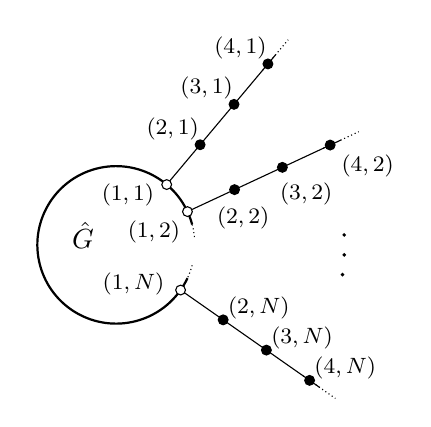
\begin{tikzpicture}[
  label distance=-5.5pt,
  thin,
  vertex/.style={circle,draw=black,fill=black,inner sep=1.25pt,
    minimum size =0mm},
  attach/.style={circle,draw=black,fill=white,inner sep=1.25pt,
    minimum size =0mm},
  dots/.style={circle,fill=black,inner sep=.5pt,
    minimum size= 0pt},
  every text node part/.style={font=\footnotesize}]

  \node at (.15, .63) [rectangle,fill=white] {$(1,1)$};
  \node at (.48, .17) [rectangle,fill=white,inner sep=0pt] {$(1,2)$};
  \node at (.22,-.5) [rectangle,fill=white] {$(1,N)$};

  \draw[thick] (15:1) arc (15:335:1);
  \draw[densely dotted] (15:1)  arc (15:5:1);
  \draw[densely dotted] (-15:1)  arc (-15:-25:1);

  \node at (-.42,.12) [rectangle] {\normalsize${\hat{G}}$};

  \foreach \x  in {50, 25,-35}{
    \draw (\x:1cm) -- (\x:3.15cm);
    \draw (\x:2.9cm) -- (\x:3.4cm) [densely dotted];
  }
  
  \node at (50:1)[attach]{};
  \node at (50:1.66)[vertex,label=150:{$(2,1)$}]{};
  \node at (50:2.33)[vertex,label=150:{$(3,1)$}]{};
  \node at (50:3)[vertex,label=150:{$(4,1)$}]{};

  \node at (25:1)[attach]{};
  \node at (25:1.66)[vertex]{};
  \node at (25:2.33)[vertex]{};
  \node at (25:3)[vertex]{};
  
  \node at (12:1.65) {$(2,2)$};
  \node at (15:2.5) {$(3,2)$};
  \node at (17.5:3.35) {$(4,2)$};

  \node at (-35:1)[attach]{};
  \node at (-35:1.66)[vertex,label=60:{$(2,N)$}]{};
  \node at (-35:2.33)[vertex,label=60:{$(3,N)$}]{};
  \node at (-35:3)[vertex,label=60:{$(4,N)$}]{};

  \node at (-2.5:2.9)[dots] {};
  \node at (2.5:2.9)[dots] {};
  \node at (-7.5:2.9)[dots] {};
\end{tikzpicture}
  \caption[Infinite used for scattering]{An infinite graph $G$ obtained from a finite graph $\widehat{G}$ by attaching $n$ semi-infinite paths. The open circles are \emph{terminals}, vertices of $\widehat{G}$ to which semi-infinite paths are attached. The internal vertices of $\widehat{G}$ are not shown.}
  \label{fig:basic_graph}
\end{figure}


%%%%
\subsubsection{Confined bound states}

The easiest states to analyze are the confined bound states, which are eigenstates in which the only nonzero amplitudes are on vertices inside the finite graph $\widehat{G}$. If any vertex on the semi-infinite paths has nonzero amplitude for some eigenstate of the Hamiltonian, then the form of the Hamiltonian forces all vertices on that path to have nonzero amplitude, and thus these confined bound states are exactly those states that have finite support in the basis of vertex states.  

To find these confined bound states, we restrict our Hilbert space to the space spanned by the internal vertices of $\widehat{G}$. The states of interest then correspond to the eigenstates of $D$ (the induced adjacency matrix of $A(G)$ when restricted to the internal vertices of $\widehat{G}$) with the additional restriction that the state lies in the nullspace of $B^\dag$, so that we can extend this state to the full Hilbert space by simply assuming all other amplitudes are zero.    

As we originally assumed that there are only $m$ internal vertices of $\widehat{G}$, there are at most $m$ such confined bound states.  Additionally, note that there are no restrictions on the eigenvalues of these states, other than those that are inherited from any restrictions placed on it by $D$ (such as the energy being bounded by the maximum degree of $\widehat{D}$).

%%%%
\subsubsection{Unconfined bound states}

The next possible type of eigenstates are those that are not confined to the finite graph $\widehat{G}$ but are still normalizable.  Since these states still have amplitude along the semi-infinite paths, we know that they must be of the form $Ae^{i k x}$, for some $A$ and $k$.  However, when $k$ is not real (corresponding to a decaying amplitude along the paths), we have that
\begin{equation}
  2 \cos(k) = 2\cos(k_r + i k_i) = 2 \cos(k_r) \cosh(k_i) - i \sin(k_r) \sinh(k_i).
\end{equation}
Hence, if we assume that the state is normalizable, then $k_i \neq 0$, and as the adjacency matrix is Hermitian, we must have that the eigenvalue is real, forcing $k_r = \pi n$ for some $n\in \NN$.  Note that this then implies that $e^{i k} = z$, for some $z\in(-1,1)\setminus\{0\}$.

As the eigenvalue equation for these states are guaranteed to be satisfied along the paths, we need to construct the form of the eigenstates inside the graph $\widehat{G}$.  We can then see that the eigenvalue equation for these vertices is given by
\begin{align}
\bigg[
  \begin{pmatrix} 
    A & B^\dag\\
    B & D
  \end{pmatrix}
  + \begin{pmatrix} 
    z \\
    0
  \end{pmatrix}
  \bigg] \begin{pmatrix}
    \vec{\alpha}\\
    \vec{\beta}
  \end{pmatrix} = \Big(z + \frac{1}{z}\Big) \begin{pmatrix} 
    \vec{\alpha}\\
    \vec{\beta}
  \end{pmatrix}
\end{align}
where $\vec{\alpha} \in \CC^N$ and $\vec{\beta}\in \CC^m$.  Note that the amplitudes for a vertex $(x,i)$ is given by $\vec{\alpha}_i z^{x-1}$.  Note that we are implicitly assuming that $\vec{\alpha} \neq \vec{0}$, for in that case we are working with a confined bound state.  

While there is no immediate reason to guess that the total number of bound states is finite, it has been shown that this number is indeed finite (see \cite{CG12} for a more thorough explanation, using Levinson's theorem for graphs).

%%%%
\subsubsection{Scattering states}

We finally reach the point of scattering states, or those unnormalizable eigenstates of the Hamiltonian.  We first assume that these states are orthogonal to all bound states, and in particular that we are orthogonal to all confined bound states, as this allows us to uniquely construct the scattering states (without this assumption, if there existed a confined bound state at the appropriate energy, then we could simply add any multiple of the confined bound state to get a different scattering state).

Taking some intuition from the classical case, we will construct a set of states that correspond to sending a particle in towards the graph $\widehat{G}$ along one of the semi-infinite paths and understanding how it scatters off of the graph.  Namely, for each $i\in[N]$ we will assume that there exists a state with amplitude along the $i$-th path of the form $e^{i k x} + S_{i,i}(k)e^{-i k x}$ for $k\in (-\pi, 0)$, and that the rest of the paths have amplitudes given by $S_{i,q}(k)e^{ikx}$.  More concretely, we assume that the form of the states is given on the infinite paths by
\begin{equation}
  \braket{x,q}{\scat_{j}(k)} = \delta_{j,q} e^{-i k x} + S_{qj} e^{i k x}.\label{eq:scattering_amplitude_paths}
\end{equation}
We then need to see whether such an eigenstate exists.  In this case, note that $S_{qj}$ corresponds to the transmitted amplitude along the $q$-th path if the particle was incident along the $j$-th path.  In the continuous case, $S$ forms a unitary matrix, which essentially means that any incoming particle must also leave, and be distinguishable from a particle incident from a different direction.  This intuition will also hold in the discrete case, but we will show this later.

If we continue to make the assumption that these states exist, we can also write the amplitudes of the $m$ interval vertices as a column vector, as $\vec{\psi}_i(k)$, in which $\vec{\psi}_{i}(k)$ is the projection of $\ket{\scat_j(k)}$ onto the internal vertices of $\widehat{G}$.  We can then collect these vectors into an $m\times N$ matrix, namely
\begin{equation}
  \Psi(k) := \begin{pmatrix} \vec{\psi}_1(k) & \vec{\psi}_2(k) & \cdots & \vec{\psi}_N(k)\end{pmatrix}
\end{equation}

Noting that the amplitudes for $\ket{\scat_j(k)}$ on the terminal vertices is given by $ e^{-i k}\delta_{j,q} + S_{qj}(k)e^{ik}$, we can then collect all of the eigenvalue equations for the vertices in $\widehat{G}$ (both internal and termal) as
\begin{equation}
  \begin{pmatrix} A & B^\dag \\
    B & D\end{pmatrix} \begin{pmatrix}  e^{-i k} \II + S(k) e^{i k}\\ \Psi(k)\end{pmatrix} 
    + \begin{pmatrix} e^{-2 i k} \II + e^{2 i k} S(k)\\ 0\end{pmatrix} = 
    2 \cos(k) \begin{pmatrix}  e^{-i k} \II + S(k) e^{i k}\\ \Psi(k)\end{pmatrix},
\end{equation}
where we have constructed the scattering matrix $S(k)$ using the scattering amplitudes $S_{qj}(k)$.

By examining the lower half of this matrix equation, we can see that
\begin{equation}
  \Psi(z) = \frac{1}{2 \cos(k) \II - D} \big( e^{-ik} B + e^{i k} B S(z)\big),
\end{equation}
which gives the amplitudes of the internal vertices in terms of the scattering matrix.  Note that we have assumed that the matrix $D$ does not have an eigenvalue equal to $2\cos(k)$, but this assumption will not be critical, as the eventual matrix $\ket{\Psi}(z)$ will be defined by analytic continuation.

Let us now examine the upper half of the matrix equation, to find
\begin{align}
  A\big(e^{-ik} \II+ e^{i k} S(k)\big) + B^\dag \Psi(k) + \big(e^{-2 ik}\II + e^{2 i k} S(z)\big) &= 2 \cos(k) \big(e^{-ik} \II + e^{i k} S(k)\big)\\
  -\Bigg(\II - e^{ik}\Big(A + B^\dag \frac{1}{2 \cos(k) - D} B\Big)\Bigg)S(k) &= \II - e^{-ik}\Big(A + B^\dag \frac{1}{2 \cos(k) - D} B\Big).
\end{align}
Hence, if we define
\begin{equation}
  Q(k) = \II - e^{ik}\Big( A + B^\dag \frac{1}{2 \cos(k) - D} B\Big),
\end{equation}
we find that
\begin{equation}
  S(k) = - Q(k)^{-1} Q(-k),
\end{equation}
if we assume that the matrix $Q(k)$ can be inverted.  Note that for all ${k\in (-\pi,0)}$, this might only be impossible for $k$ in which $D$ has a $2\cos(k)$ eigenvalue, in which case we have already run into a problem with the definition of $\Psi(k)$.

Putting this all together, we then have that the states $\ket{\scat_j(k)}$ exist for all $k\in (-\pi,0)$ for which $D$ does not have a $2\cos(k)$ eigenvalue.  We will see in \sec{def_of_gamma_matrix} that this restriction is an artifact of our construction of $S(k)$, and thus the scattering states will be well defined for all $k\in (-\pi,0)$.


%%%%
\subsubsection{Half-bound states}

As a limiting case for both the scattering states and the unconfined bound states, we have those states with $k = 0$ or $k= \pi$ (or equivalently with $z = \pm 1$).  In either case, the two momenta correspond to particles that don't move, but the states themselves are not normalizable.  They won't play much of a role in this thesis, but I did want to mention them.


%%%%
\subsubsection{Scattering states for all $k$}\label{sec:def_of_gamma_matrix}

While the above construction is a useful definition of the scattering states for most ${k\in(-\pi,0)}$, unfortunately there are specific values of $k$ (namely those for which $D$ has eigenvalue $2\cos(k)$) in which the above analysis doesn't hold, due to the singularity of particular matrices.  If we want to show that these scattering states exist for all $k\in (-\pi,0)$, we need to somehow show that these singularities are just a problem of the analysis and are not intrinsic barriers to existence.  Note that this construction closely follows that of \cite{CG12}.

Along these lines, let us extend our analysis to complex $z$, instead of only focusing on amplitudes of the form $e^{ik}$.  We will define the matrix
\begin{equation}
  \gamma(z) := \begin{pmatrix}  z A - \II & z B^\dag\\
    z B & zD - (1+z^2) \II\end{pmatrix}.
    \label{eq:gamma_def}
\end{equation}
This matrix is closely related to the eigenvalue equation for vertices of the graph $\widehat{G}$, but with $e^{ik}$ replaced with $z$.  

With this definition, it will be useful to note the following matrix equalities.  In particular, assuming that $z$ is a complex number such that the following matrices are not singular, we have:
\begin{align}
  \begin{pmatrix} \II & zB^\dag\\
    0 & z D - (1+ z^2) \II \end{pmatrix}
    \begin{pmatrix} - Q(z) & 0\\
      \frac{z}{zD - (1+ z^2)\II}B & \II\end{pmatrix} 
      &= \begin{pmatrix} -Q(z) + z B^\dag \frac{1}{D - (z + z^{-1})} B & z B^\dag\\
        zB & zD - (1+z^2)\II\end{pmatrix} \\
        &= \gamma(z)
\end{align}
Additionally, if we note that the inverse of a block diagonal matrix can be written as
\begin{equation}
  \begin{pmatrix} X & Y \\
  Z & W\end{pmatrix}^{-1} = \begin{pmatrix} \big(X - Y W^{-1} Z\big)^{-1} & - X^{-1} Y \big(W - Z X^{-1} Y\big)^{-1}\\
    - W^{-1} Z \big(X - Y W^{-1} Z\big)^{-1} & \big(W - Z X^{-1} Y\big)^{-1}\end{pmatrix},
\end{equation}
we can then invert this equation for $\gamma(z)$ as 
\begin{align}\gamma(z)^{-1} &= \begin{pmatrix} - Q(z) & 0\\
      \frac{z}{zD - (1+ z^2)\II}B & \II\end{pmatrix}^{-1} \begin{pmatrix} \II & zB^\dag\\
    0 & z D - (1+ z^2) \II \end{pmatrix}^{-1}\\
    &= \begin{pmatrix}
      - Q(z)^{-1} & 0\\
      \frac{z}{z D - (1+z^2)\II} B Q(z)^{-1} & \II
    \end{pmatrix}
    \begin{pmatrix}
      \II & - B^{\dag} \frac{z}{zD - (1+z^2)\II}\\
      0 & \frac{1}{zD - (1+z^2)\II}
    \end{pmatrix}.
\end{align}
Combining these two matrix equations, we can then find that
\begin{align}
  \gamma (z)^{-1} \gamma(z^{-1}) &= \begin{pmatrix}
      - Q(z)^{-1} & 0\\
      \frac{z}{z D - (1+z^2)\II} B Q(z)^{-1} & \II
    \end{pmatrix}
    \begin{pmatrix}
      \II & - B^{\dag} \frac{z}{zD - (1+z^2)\II}\\
      0 & \frac{1}{zD - (1+z^2)\II}
    \end{pmatrix}\nonumber\\
  &\qquad \qquad \times
    \begin{pmatrix} \II & z^{-1}B^\dag\\
    0 & z^{-1} D - (1+ z^{-2}) \II \end{pmatrix}
    \begin{pmatrix} - Q\big(z^{-1}\big) & 0\\
      \frac{z^{-1}}{z^{-1}D - (1+ z^{-2})\II}B & \II\end{pmatrix} \\
  &=  \begin{pmatrix}
      - Q(z)^{-1} & 0\\
      \frac{z}{z D - (1+z^2)\II} B Q(z)^{-1} & \II
    \end{pmatrix}
    \begin{pmatrix}
      \II & 0\\
      0 &z^{-2}\II \end{pmatrix}
    \begin{pmatrix} - Q\big(z^{-1}\big) & 0\\
      \frac{z^{-1}}{z^{-1}D - (1+ z^{-2})\II}B & \II\end{pmatrix} \\
   &= \begin{pmatrix}
      - Q(z)^{-1} & 0\\
      \frac{z}{z D - (1+z^2)\II} B Q(z)^{-1} &z^{-2} \II
    \end{pmatrix}
    \begin{pmatrix} - Q\big(z^{-1}\big) & 0\\
      \frac{z^{-1}}{z^{-1}D - (1+ z^{-2})\II}B & \II\end{pmatrix} \\
  &= \begin{pmatrix}
      Q(z)^{-1}Q(z^{-1}) & 0\\
      \frac{1}{D - (z+z^{-1})\II }B \big(z^{-2} \II - Q(z)^{-1}Q(z^{-1}) \big) & z^{-2}\II
    \end{pmatrix}\\
  &= -\begin{pmatrix}
      S(z) & 0\\
     z^{-1} \Psi(s) & -z^{-2}\II
    \end{pmatrix},\label{eq:gamma_gives_S}
\end{align}
where we have extended the definition of $S$ and $\Psi$ to all complex $z$ instead of just $e^{ik}$

With these matrix equations, we have a representation of the scattering matrix and the interior amplitudes in terms of the matrix $\gamma$.  If we then note that
\begin{equation}
  \gamma(z)^{-1} = \frac{1}{\det \gamma(z)} \adj \gamma (z)
\end{equation}
where $\adj \gamma (z)$ is the adjugate matrix of $\gamma(z)$, then by \eq{gamma_gives_S} we can then see that the entries of $\gamma(z)$, and thus the entries of $S(z)$ and $\Psi(z)$, are rational functions of $z$. 

With this fact, to show that the problems defining the states $\ket{\scat_j(k)}$ are a result of our analysis rather than intrinsic difficulties, we need only show that there are no poles in the matrix elements for $S(z)$ or $\Psi(z)$ for $z$ on the unit circle.  We actually have that for all such $z$, there is an upper bound on the norm of the scattering amplitudes, which might depend on the graph $\widehat{G}$.
\begin{lemma}
Given $\widehat{G}$, there exists a constant $\lambda\in\mathbb{R}$ such that $|\langle v|sc_{j}(k)\rangle|<\lambda$ for all $k\in[-\pi,\pi)$, $j\in\{1,\ldots,N\}$, and $v\in\widehat{G}$.
\end{lemma}\label{lem:scattering_state_amplitude_bound}

\begin{proof}
Note that 
\begin{equation}
\gamma\left(\frac{1}{z}\right)=\frac{1}{z^{2}}\gamma(z)+\left(\frac{1}{z^{2}}-1\right)\widehat{P}\end{equation}
where 
\begin{equation}
\widehat{P}=\begin{pmatrix}
1 & 0\\
0 & 0\end{pmatrix}
\end{equation}
projects onto the $N$ vertices of $\widehat{G}$ attached to semi-infinite paths. Hence 
\begin{equation}
-\gamma(z)^{-1}\gamma\left(\frac{1}{z}\right)=-\frac{1}{z^{2}}+\left(1-\frac{1}{z^{2}}\right)\gamma(z)^{-1}\widehat{P}.
\end{equation}

Let $\{|\psi_{c}\rangle \colon c\in\{1,\ldots,n_{c}\}\}$ be eigenstates of $\widehat{H}$ satisfying $\widehat{P}|\psi_c\rangle=0$, and let this set be an orthonormal basis for the span of all such states. Then
 \begin{equation}
\left(1-\frac{1}{z^{2}}\right)\gamma(z)^{-1}\widehat{P}=\left(1-\frac{1}{z^{2}}\right)\left(1-\sum_{j=1}^{n_{c}}|\psi_{c}\rangle\langle\psi_{c}|\right)\gamma(z)^{-1}\left(1-\sum_{j=1}^{n_{c}}|\psi_{c}\rangle\langle\psi_{c}|\right)\widehat{P}\end{equation}
 since each $|\psi_c\rangle$ is an eigenvector of $\gamma(z)$ and
$\widehat{P}|\psi_{c}\rangle=0$. Reference \cite{CG12} shows (in Part 2 of the proof of Theorem 1) that
\begin{equation}
\det\left(\frac{1}{1-z^{2}}\right)M(z)\neq0\text{ for }|z|=1,
\end{equation}
where $M(z)$ is the $(N+m-n_{c})\times(N+m-n_{c})$ matrix of $\gamma(z)$ in the subspace of states orthogonal to the span of $\{|\psi_{c}\rangle \colon c\in\{1,\ldots,n_{c}\}\}$. Therefore 
\begin{align*}
\frac{1}{z}\langle v|\mathrm{sc}_{j}(k)\rangle & =  -\langle v|\gamma(z)^{-1}\gamma\left(\frac{1}{z}\right)|j\rangle\\
 & = \langle v|\left(1-\frac{1}{z^{2}}\right)\left(1-\sum_{j=1}^{n_{c}}|\psi_{c}\rangle\langle\psi_{c}|\right)\gamma(z)^{-1}\left(1-\sum_{j=1}^{n_{c}}|\psi_{c}\rangle\langle\psi_{c}|\right)|j\rangle
\end{align*}
has no poles on the unit circle, and the result follows.

\end{proof}

As such, we have that the scattering states are well defined for all $k\in (-\pi,0)$.  


%%%%%%%%%%%%%%%
\subsection{Scattering matrix properties}

While the use of the $\gamma$ matrix gives an explicit construction of the form of the eigenstates on the internal vertices, the alternate definition in terms o the $Q$ matrix can be used to easily show several properties of the scattering matrix.  In particular, remember that
\begin{equation}
  S(k) = - Q(z)^{-1} Q(z^{-1}),
\end{equation}
where $z=e^{i k}$, and the matrices $Q(z)$ are given by
\begin{equation}
  Q(z) = \II - z \Big( A + B^\dag \frac{1}{ \frac{1}{z} + z - D} B\Big).
\end{equation}
Note that $Q(z)$ and $Q(z^{-1})$ commute for all $z\in \CC$, as they can both be written as $\II + z H(z + z^{-1})$.

Using this expression for the scattering matrix, it is easy to see that $S(k)$ is a unitary matrix, as 
\begin{equation}
  S(k)^{\dag} = - Q(z^{-1})^\dag (Q(z)^{-1})^\dag
\end{equation}
and that
\begin{equation}
  Q(z)^\dag = \II^\dag - z^\dag\Big( A^\dag + B^\dag \Big(\frac{1}{\frac{1}{z} + z - D}\Big)^\dag (B^\dag)^\dag\Big) 
     = \II - z^\dag \Big(A + B^\dag \frac{1}{\frac{1}{z^\dag} + z^\dag - D} B \Big) = Q(z^\dag)
\end{equation}
and thus
\begin{equation}
  S(k)^\dag = -Q(z^{-1})^\dag (Q(z)^{-1})^\dag = - Q(z) Q(z^{-1})^{-1} = Q(z^{-1})^{-1} Q(z) = S(k)^{-1}
\end{equation}
where we used the fact that $z=e^{ik}$ so that $z^\dag = z^{-1}$, and the fact that $Q(z)$ and $Q(z^{-1})$ commute.

Additionally, we can make use of the fact that $S$ is derived from an unweighted graph to show that the scattering matrices are symmetric.  In particular, note that $Q(z)$ is symmetric for all $z$, since $D$ is symmetric, symmetric matrices are closed under inversion, $A$ is symmetric and $B$ is a 0-1 matrix.  As such, we have that
\begin{align}
  S(k)^T &= -\big( Q(z)^{-1} Q(z^{-1})\big)^T = -Q(z^{-1})^T (Q(z)^{-1})^T \\
    &= -Q(z^{-1}) Q(z)^{-1} = -Q(z)^{-1} Q(z^{-1}) = S(k)
\end{align}
where we used the fact that $Q(z)$ and $Q(z^{-1})$ commute.

Putting this together, we have that $S(k)$ is a symmetric, unitary matrix for all $k$.

%%%%%%%%%%%%%%%%%
\subsection{Orthonormality of the scattering states}

We now have some basic ideas behind the scattering behavior.  In particular, we have that the scattering states exist for all $k$, and that the scattering matrices are symmetric and unitary.  However, one of the most important behaviors we need is that the scattering states are orthonormal, and that they form a basis for the Hilbert space corresponding to the graph. 

We will first show that two scattering states are orthonormal.

\begin{lemma}
  Let 	$k,p\in (-\pi,0)$, and let $i,j\in [N]$.  We then have that
  \begin{align}
    \braket{\scat_i(p)}{\scat_{j}(k)} = \frac{1}{2\pi} \delta_{i,j} \delta(p-k),
    \label{eq:delta}
  \end{align}
  where the two sides are equal as functionals against integration.
\label{lem:orthonormality_of_scattering_states}
\end{lemma}
\begin{proof}
Let 
\begin{align}
\Pi_{1} & = \sum_{x=1}^{\infty}\sum_{q=1}^{N}|x,q\rangle\langle x,q|%\\
&\Pi_{2} & = \mathbb{I}-\sum_{x=2}^{\infty}\sum_{q=1}^{N}|x,q\rangle\langle x,q|%\\
&\Pi_{3} & = \sum_{q=1}^{N}|1,q\rangle\langle1,q|.\end{align}
First write 
\begin{align*}
\langle\mathrm{sc}_{i}(p)|\Pi_{1}|\mathrm{sc}_{j}(k)\rangle & = \sum_{x=1}^{\infty}\sum_{q=1}^{N}(\delta_{iq}e^{ipx}+S_{qi}^{\ast}(p)e^{-ipx})(\delta_{jq}e^{-ikx}+S_{qj}(k)e^{ikx})\\
 & = \frac{1}{2}\left(\delta_{ij}+\sum_{q=1}^{N}S_{qi}^{\ast}(p)S_{qj}(k)\right)\left(\sum_{x=1}^{\infty}e^{i(p-k)x}+\sum_{x=1}^{\infty}e^{-i(p-k)x}\right)\\
 & \quad +\frac{1}{2}\left(\delta_{ij}-\sum_{q=1}^{N}S_{qi}^{\ast}(p)S_{qj}(k)\right)\left(\sum_{x=1}^{\infty}e^{i(p-k)x}-\sum_{x=1}^{\infty}e^{-i(p-k)x}\right)\\
 & \quad +\frac{1}{2}(S_{ji}^{\ast}(p)+S_{ij}(k))\left(\sum_{x=1}^{\infty}e^{-i(p+k)x}+\sum_{x=1}^{\infty}e^{i(p+k)x}\right)\\
 & \quad +\frac{1}{2}(S_{ji}^{\ast}(p)-S_{ij}(k))\left(\sum_{x=1}^{\infty}e^{-i(p+k)x}-\sum_{x=1}^{\infty}e^{i(p+k)x}\right).\end{align*}
We use the following identities for $p,k\in(-\pi,0)$: 
\begin{align*}
\sum_{x=1}^{\infty}e^{i(p-k)x}+\sum_{x=1}^{\infty}e^{-i(p-k)x} & = 2\pi\delta(p-k)-1 \\
\sum_{x=1}^{\infty}e^{i(p+k)x}+\sum_{x=1}^{\infty}e^{-i(p+k)x} &=-1 \\
\sum_{x=1}^{\infty}e^{i(p-k)x}-\sum_{x=1}^{\infty}e^{-i(p-k)x} & = i\cot\left(\frac{p-k}{2}\right) \\
\sum_{x=1}^{\infty}e^{i(p+k)x}-\sum_{x=1}^{\infty}e^{-i(p+k)x} &= i\cot\left(\frac{p+k}{2}\right).
\end{align*}
These identities hold when both sides are integrated against a smooth function of $p$ and $k$. Substituting, we get
\begin{align}
\langle\mathrm{sc}_{i}(p)|\Pi_{1}|\mathrm{sc}_{j}(k)\rangle & =  2\pi\delta_{ij}\delta(p-k)+\delta_{ij}\left(\frac{i}{2}\cot\left(\frac{p-k}{2}\right)-\frac{1}{2}\right)\nonumber\\
&\quad+\sum_{q=1}^{N}S_{qi}^{\ast}(p)S_{qj}(k)\left(-\frac{i}{2}\cot\left(\frac{p-k}{2}\right)-\frac{1}{2}\right)\nonumber \\
 &\quad+S_{ji}^{\ast}(p)\left(-\frac{1}{2}-\frac{i}{2}\cot\left(\frac{p+k}{2}\right)\right)\nonumber\\
&\quad+S_{ij}(k)\left(-\frac{1}{2}+\frac{i}{2}\cot\left(\frac{p+k}{2}\right)\right)\label{eq:pi1}
\end{align}
where we used unitarity of the $S$-matrix to simplify the first term.
Now turning to $\Pi_{2}$ we have \begin{equation}
\langle\mathrm{sc}_{i}(p)|H\Pi_{2}|\mathrm{sc}_{j}(k)\rangle=2\cos(p)\langle\mathrm{sc}_{i}(p)|\Pi_{2}|\mathrm{sc}_{j}(k)\rangle\end{equation}
 and 
\begin{align*}
\langle\mathrm{sc}_{i}(p)|H\Pi_{2}|\mathrm{sc}_{j}(k)\rangle & = \langle\mathrm{sc}_{i}(p)|\bigg(2\cos(k)\Pi_{2}|\mathrm{sc}_{j}(k)\rangle+\sum_{q=1}^{N}(e^{-ik}\delta_{qj}+S_{qj}(k)e^{ik})|2,q\rangle\\
&\quad -\sum_{q=1}^{N}(e^{-2ik}\delta_{qj}+S_{qj}(k)e^{2ik})|1,q\rangle\bigg).
\end{align*}
 Using these two equations we get 
\begin{align*}
(2\cos(p)-2\cos(k))\langle\mathrm{sc}_{i}(p)|\Pi_{2}|\mathrm{sc}_{j}(k)\rangle & =  \delta_{ij} (e^{2ip-ik}-e^{-2ik+ip})+S_{ji}^{\ast}(p)(e^{-2ip-ik}-e^{-2ik-ip})\\
 & \quad +S_{ij}(k)(e^{2ip+ik}-e^{2ik+ip})\\
& \quad +\sum_{q=1}^{N}S_{qi}^{\ast}(p)S_{qj}(k)(e^{-2ip+ik}-e^{2ik-ip}).
\end{align*}
 Noting that
\begin{equation}
\langle\mathrm{sc}_{i}(p)|\Pi_{3}|\mathrm{sc}_{j}(k)\rangle=\sum_{q=1}^{N}(\delta_{iq}e^{ip}+S_{qi}^{\ast}(p)e^{-ip})(\delta_{jq}e^{-ik}+S_{qj}(k)e^{ik}),
\end{equation}
we have 
\begin{align}
\langle\mathrm{sc}_{i}(p)|\Pi_{2}-\Pi_{3}|\mathrm{sc}_{j}(k)\rangle & = \delta_{ij}\left(\frac{e^{2ip-ik}-e^{-2ik+ip}}{2\cos(p)-2\cos(k)}-e^{ip-ik}\right)\nonumber\\
&\quad+S_{ji}^{\ast}(p)\left(\frac{e^{-2ip-ik}-e^{-2ik-ip}}{2\cos(p)-2\cos(k)}-e^{-ip-ik}\right)\nonumber \\
 & \quad +S_{ij}(k)\left(\frac{e^{2ip+ik}-e^{2ik+ip}}{2\cos(p)-2\cos(k)}-e^{ip+ik}\right)\nonumber\\
&\quad+\sum_{q=1}^{N}S_{qi}^{\ast}(p)S_{qj}(k)\left(\frac{e^{-2ip+ik}-e^{2ik-ip}}{2\cos(p)-2\cos(k)}-e^{-ip+ik}\right)\nonumber \\
  & = \delta_{ij}\left(\frac{1}{2}-\frac{i}{2}\cot\left(\frac{p-k}{2}\right)\right)+S_{ji}^{\ast}(p)\left(\frac{1}{2}+\frac{i}{2}\cot\left(\frac{p+k}{2}\right)\right)\nonumber\\
&\quad+S_{ij}(k)\left(\frac{1}{2}-\frac{i}{2}\cot\left(\frac{p+k}{2}\right)\right)\nonumber\\
&\quad+\sum_{q=1}^{N}S_{qi}^{\ast}(p)S_{qj}(k)\left(\frac{1}{2}+\frac{i}{2}\cot\left(\frac{p-k}{2}\right)\right).
\label{eq:pi2_pi3}
\end{align}
 Adding equation \eq{pi1} to equation \eq{pi2_pi3} gives
equation \eq{delta}.
\end{proof}

With the fact that the scattering states are orthogonal, it will also be useful to see that they form an orthonormal basis for the Hilbert space.  In particular, Childs and Gosset showed in \cite{CG12} that this holds.  Assuming that the confined bound states were spanned by the orthonormal states $\{\ket{\psi_c} : c\in [n_c]\}$ and that the orthogonal bound states are spanned by the orthonormal basis $\{\ket{\phi_b} : b \in [n_b]\}$, they showed the following theorem:

\begin{theorem}[Theorem 1 of \cite{CG12}] Let $v$ and $w$ be any two vertices of the graph $G$.  Then
\begin{align}
  \bra{v} \bigg[ \int_{-\pi}^0 \frac{dk}{2\pi} \ketbra{\scat_j(k)}{\scat_j(k)} + \sum_{b= 1}^{n_b} \ketbra{\phi_b}{\phi_b}  + \sum_{c=1}^{n_c} \ketbra{\psi_c}{\psi_c} \bigg] \ket{w} = \delta_{v,w}.
\end{align}
\label{thm:scat_basis}
\end{theorem}

Most of our results will be in regards to the scattering states, but having this decomposition of the identity will allow us to show better bounds.  In particular, we will be able to guarantee that certain states have almost no support on states other than scattering states.

%\section{Applications of graph scattering}
%
%While graph scattering is a relatively new area of study, it has found several applications.  As the behavior of a scattered particle is heavily dependent on both the momentum and the graph used for scattering, we can use the scattering behavior as a probe of properties about the graph, as well as a kind of probe for the momentum of the incoming particle.  In particular, if we know the momentum of a wave-packet, we can determine the scattering amplitudes to gain information about the graph, such as whether it has eigenstates at particular momentum.  If we know a graphs scattering behavior, we can then use the scattering to check whether a wave-packet has a desired momentum, and then do something to the particular wave-packet.
%
%\subsection{NAND Trees}
%
%The original motivating idea for understanding graph scattering was an oracular separation between quantum and classical computation, for a problem involving NAND trees.  In particular, Edward Fahri, Jeffrey Goldstone, and Sam Gutmann gave a scattering algorithm \cite{FGG08} for this problem that was provably faster than any classical algorithm.
%
%A NAND tree is a function on $N$ variables, where $N$ is a power of two, such that the value of the leaves are given by the input to the function, while each parent node's value is given by the NAND of its children's values.  The NAND tree problem is then to evaluate the root.  
%
%Now for any oracular problem, we are given black-box access to the input, and want to minimize the total number of queries to the input.  In particular, the actual runtime of an algorithm generally is not measured, and instead we simply count the number of bits of the input the algorithm accesses.  While this might not always give a realistic gauge for the time a particular problem takes to solve, it does allow for information theoretic bounds on the number of queries.  In particular, oracular problems often allow us to guarantee that any algorithm will require a certain number of queries in order to solve the problem.
%
%If we perform an analysis on the NAND tree problem, any deterministic algorithm will require $N$ queries in order to evaluate the root, as in the worst case we will need to examine every bit of the input.  However, if we instead work with probabilistic computation, there is a randomized algorithm \cite{SW86} that can solve this problem in $\OO(N^\alpha)$ time, where $\alpha = \log_2(1 + \sqrt{33}) - 2 \approx 0.753$.  Additionally, any randomized algorithm will require this many queries \cite{San95}.  Fahri, Goldstone, and Gutmann were able to construct a quantum algorithm that solves the NAND tree using only $\OO(\sqrt{N})$ queries, which is provably better than in the classical case.
%
%The reason that we are interested in this is that the original algorithm uses graph scattering explicitly.  In particular, a binary tree is attached to an infinite path at the root, and then additional vertices are attached to the leaves depending on whether the binary value is 0 or 1.  It turns out that at energy 0 (i.e., momentum $-\pi/2$), such a tree has perfect transmission from one path to the other if the tree evaluates to 1, and perfect reflection if the tree evaluates to 0.  Hence, if a wave packet with momentum centered around $-\pi/2$ is scattered off of such a graph, by determining the location of the particle after it has scattered we evaluate the tree. 
%
%In this case, the requisite size of the wave-packet turns out to be $\OO(\sqrt{N})$, and thus this amount of time is required in order for the scattering to occur.  The total evolution time is closely related to the number of queries that the algorithm uses during the computation, and thus this is a quantum algorithm that has a provable advantage over classical computing.


%%%%%%%%%%%%%%%%%%%%%%%%%%%%%%%%%%%%%%%%%%%%%%%%%%%%%%%%%%%%%%%
\section{Wavepacket scattering}

Up until this point, we have taken as intuition that the scattering states correspond to an incoming wave packet at some momentum, and then scatterings with a corresponding $S$-matrix.  However, this is somewhat weird, in that the scattering states are eigenstates of the Hamiltonian, and thus do not change over time, while scattering states explicitly move.  

In this section, we will show that our intuitive naming is useful.  In particular, we will show that preparing a wave packet centered at some momenta will scatter as the $S$-matrix of the corresponding scattering state.  Further, the shape of the wave packet will remain approximately the same.

In \cite{MPQW}, Childs, Gosset, and W. proved a nice bound on the time-evolution of square wave packets.  These approximations were useful as the necessary mathematics involved in proving the related bounds only involved unweighted sums of amplitudes that were identical to the eigenstates of the corresponding Hamiltonians.  In particular, they were able to prove the following bound:
\begin{theorem}[Childs, Gosset, W.\cite{MPQW}]
Let $\widehat{G}$ be an $(N+m)$-vertex graph. Let $G$ be a graph obtained from $\widehat{G}$ by attaching semi-infinite paths to $N$ of its vertices, and let $S$ be the corresponding S-matrix.  Let $k\in(-\pi,0)$, $M,L\in\NN$, $j\in\{1,\ldots,N\}$, and
\begin{equation}
  |\psi^{j}(0)\rangle=\frac{1}{\sqrt{L}}\sum_{x=M+1}^{M+L}e^{-ikx}|x,j\rangle.
\end{equation}
Let $c_{0}$ be a constant independent of $L$. Then, for all $0\leq t\leq c_{0}L$,
\begin{equation}
  \left\Vert e^{-iA(G) t}|\psi^{j}(0)\rangle-|\alpha^{j}(t)\rangle\right\Vert =\OO(L^{-{1}/{4}})
\end{equation}
where 
\begin{align}
  |\alpha^{j}(t)\rangle & =  \frac{1}{\sqrt{L}}e^{-2it\cos k}\sum_{x=1}^{\infty}\sum_{q=1}^{N}\left(\delta_{qj} e^{-ikx}R(x-\left\lfloor 2t\sin k\right\rfloor)+S_{qj}(k)e^{ikx}R(-x-\left\lfloor 2t\sin k\right\rfloor)\right)|x,q\rangle
\end{align}
with
\begin{align}
R(l) & =  \begin{cases}
1 & \text{if }l\in\{M+1,M+2,\ldots,M+L\}\\
0 & \text{otherwise.}\end{cases}
\end{align}
\end{theorem}

While these bounds were sufficient for the purposes of their paper, as they only required polynomial versus exponential overhead, the bounds they proved where not the best possible.  Their use of square approximations was most likely not optimal in terms of the resulting errors.  

As such, this section is devoted to proving a corresponding bound on the scattering behavior of a Gaussian wave packet, instead of square wave packets.  We prove near quadratically better bounds than those of \cite{MPQW} in regards to the single-particle scattering, as the Guassian wave packets have nice dispersion properties, but unfortunately the proof becomes a little more complicated.  In particular, we prove the following lemma:
\begin{theorem}
  Let $\widehat{G}$ be an $(N+m)$-vertex graph, let $G$ be the graph obtained from $\widehat{G}$ by attaching $N$ semi-infinite paths to the first $N$ of its vertices, and let $S$ be the corresponding $S$-matrix.  Let $\ket{\psi_j(0)}$ be a cut-off Gaussian distribution with momentum $k$ and standard deviation $\sigma$ centered at $\mu$, with the cut-off at a distance $L$ from the center.  Namely, let 
  \begin{equation}
    \ket{\psi^j(0)} = \gamma \sum_{x = \mu - L}^{\mu + L} e^{- i k x} e^{- (x - \mu)^2/2\sigma^2} \ket{x,j}  \label{eq:guass_start_defn},
  \end{equation}
  where $\gamma$ is the normalization of $\ket{\psi^j(0)}$.  Then let us define the state 
  \begin{align}
    \ket{\alpha^j(t)} &= \gamma e^{-2 i t \cos k} \Bigg[ \sum_{x = \max\{\mu(t) -L,1\}}^{\max\{\mu(t)+L,0\}} e^{-i k x} e^{ -(x - \mu(t))^2/2\sigma^2} 
    			 \ket{x,j} \nonumber\\
			  &\qquad\qquad\qquad+ \sum_{x = \max\{-\mu(t)-L,1\}}^{\max\{-\mu(t) + L,0\}} \sum_{q=1}^N  S_{qj}(k) e^{i k x} e^{-(x + \mu(t))^2/2\sigma^2} \ket{x,q} \Bigg]\label{eq:guass_approximation_defn}
  \end{align}
  where
  \begin{equation}
    \mu(t) = \mu - \lceil 2 t \sin(k)\rceil.
  \end{equation}
  If $\sigma = c_1 \frac{ L}{\sqrt{\log L}}$ for some constant $c_1 < \frac{1}{\sqrt{2}}$, we then have that for $0 < t < c_2 L$,  
  \begin{equation}
    \norm{e^{-i A(G) t} \ket{\psi^j(0)} - \ket{\alpha^j (t)}} \in \OO \bigg(\sqrt{\frac{\log L}{L}} \bigg).,
  \end{equation}  
\label{thm:single_particle_wavepacket_bound}
\end{theorem}

Note that this bound is extremely similar to that of \cite{MPQW}, albeit with a slightly more complicated definition for the approximate state.  However, when the wave packet is far from the 






\subsection{Jacobi $\Theta$-function}

Before we delve into the proof of the wavepacket scattering, it will be useful to define a kind of discrete approximation to a Gaussian.  In particular, let us define the function
\begin{equation}
  h_L^\sigma(\phi) = \sum_{n = -L}^L e^{i \phi n} e^{-\frac{ x^2}{2\sigma^2}}. 
  \label{eq:h_L_defn}
\end{equation}
This is closely related to the amplitude of the original wavepacket in \thm{single_particle_wavepacket_bound}, and will be used extensively in our proof.

Additionally, this function is closely related to the Jacobi theta function, for which we refer the reader to Chapter 10 of \cite{SSCA} for a broad overview.  This function, $\Theta(z,q)$ is defined for all complex $z$ and all $q$ with positive imaginary part as
\begin{equation}
  \Theta(z,q) = \sum_{n = -\infty}^\infty e^{ \pi i n^2 \tau} e^{ 2\pi  i n z}
\end{equation}
 and is related to our $h$ as 
\begin{equation}
  h_{\infty}^\sigma(\phi) = \sum_{n = -\infty}^\infty e^{ i \phi n} e^{ - \frac{ n^2}{2\sigma^2}} = \Theta\Bigg(\frac{\phi}{2\pi}, \frac{i}{2\pi \sigma^2} \Bigg).
\end{equation}
The Jacobi theta function has several symmetries, such as the fact that $\Theta(z,q) = \Theta(-z, q)$, and one that is similar to the Fourier transform.  In particular, using our language and Theorem 1.6 from Chapter 10 of \cite{SSCA}, we have
\begin{equation}
  h_{\infty}^\sigma (\phi) = \Theta\Bigg(\frac{\phi}{2\pi}, \frac{i}{2\pi \sigma^2} \Bigg) = \sqrt{2\pi} \sigma e^{ - \frac{\sigma^2\phi^2}{2}} \Theta \big(i \phi\sigma^2, 2\pi i \sigma^2 \big) =  \sqrt{2\pi} \sigma e^{ - \frac{\sigma^2\phi^2}{2}}  h_{\infty}^{1/(2\pi \sigma)}\big(2\pi i \phi \sigma^2 \big).
  \label{eq:discrete_fourier_transform}
\end{equation}
This can be viewed as a discrete version of a Fourier transform, as the summand goes from a Gaussian distribution with standard deviation $\sigma$ to one that has standard deviation proportional to $\sigma^{-1}$ along with an exponential suppression term.  Additionally, note that the argument to the $h$ function is now complex, but we will only use such terms when dealing with the full infinite sum.


Let us now give some bounds on the various norms of $h_L^\sigma$, where some of our bounds where found in \cite{Cook09}.  These will assist us greatly in our proof of the theorem.  Assuming that $L > 0$, and that $\phi$ is real, we have that
\begin{align}
  \big|h_{\infty}^{\sigma}(\phi) - h_{L}^{\sigma}(\phi) \big| &= \Big| \sum_{n=L+1}^\infty 2 \cos (n\phi) e^{- \frac{n^2}{2\sigma^2}}\Big|\\
   &\leq 2 \sum_{n = L+1}^\infty e^{ -\frac{n^2}{2\sigma^2}}\\ 
   &\leq 2 \int_{L}^\infty e^{- \frac{x^2}{2\sigma^2}} dx\\
   &= 2 \sigma \int_{L/\sigma}^\infty e^{- \frac{u^2}{2}}{du}\\
   &< 2 \sigma \int_{L/\sigma}^\infty \frac{\sigma u}{L} e^{-\frac{u^2}{2}} du\\
   &= \frac{2 \sigma^2}{L} e^{- \frac{L^2}{2\sigma^2}},
\end{align}
while if $L = 0$ we instead have
\begin{align}
  \big|h_{\infty}^{\sigma}(\phi) - 1 \big| &= \Big| \sum_{n=1}^\infty 2 \cos (n\phi) e^{- \frac{n^2}{2\sigma^2}}\Big|\\
   &\leq 2e^{- \frac{1}{2\sigma^2}} +  \sum_{n = 2}^\infty e^{ -\frac{n^2}{2\sigma^2}}\\ 
   &\leq 2e^{- \frac{1}{2\sigma^2}} + 2 \int_{1}^\infty e^{- \frac{x^2}{2\sigma^2}} dx\\
   &< 2 e^{- \frac{1}{2\sigma^2}} +  2\sigma^2 e^{-\frac{1}{2\sigma^2}}\\
   &= 2(1+ \sigma^2) e^{-\frac{1}{2\sigma^2}}.
\end{align}
In addition, if $\phi$ is complex, We will now try to bound the size of $h_\infty^\sigma(\phi)$, for small (but real) $\sigma$ and imaginary $\phi$ (so as to use the discrete Fourier transform).  In particular, if we assume that $\phi = \phi_r + i \phi_i$ and that $1 > \sigma^2 |\phi_i|$, we will have
\begin{align}
  \big|h_\infty^\sigma(\phi) - 1\big| &= \bigg|\sum_{n=1}^\infty 2 \cos(n \phi) e^{-\frac{n^2}{2\sigma^2}}\Bigg|\\
    &\leq   4 e^{- \frac{1}{2\sigma^2} + |\phi_i|} + 4 e^{ \frac{\sigma^2|\phi_i|^2 }{2}}\sum_{n=2}^\infty \exp\Big[ -\frac{1}{2}\Big(\frac{n}{\sigma} - \sigma |\phi_i|\Big)^2 \Big]\\
    &< 4 e^{ - \frac{1}{2\sigma^2} + |\phi_i|} + 4 e^{ \frac{\sigma^2|\phi_i|^2 }{2}}\int_{1}^\infty  \exp\Big[ -\frac{1}{2}\Big(\frac{x}{\sigma} - \sigma |\phi_i|\Big)^2 \Big]dx\\
    &< 4 e^{-\frac{1}{2\sigma^2} + |\phi_i|} + \frac{4 \sigma e^{\frac{\sigma^2|\phi_i|^2}{2}}}{\frac{1}{\sigma} - \sigma |\phi_i|} \int_{\frac{1}{\sigma} - \sigma|\phi_i|}^\infty u e^{-\frac{u^2}{2}} du\\
    &=  4 e^{-\frac{1}{2\sigma^2} + |\phi_i|} + \frac{4 \sigma}{\frac{1}{\sigma} - \sigma |\phi_i|} e^{-\frac{1}{2\sigma^2} + |\phi_i|}\\
    &= 4 \Big[1 + \frac{\sigma^2}{1 - \sigma^2 |\phi_i|} \Big]e^{-\frac{1}{2\sigma^2} + |\phi_i|} .
\end{align}

We can then collect these bounds into a lemma, which we will reference several times in the thesis.
\begin{lemma}
\label{lem:h_bounds}
  Let $h_L^\sigma(\phi)$ be defined as above.  For any real $\phi$, and $L>0$, we have that
  \begin{align}
    \big| h_\infty^\sigma(\phi) - h_L^\sigma(\phi)\big| < \frac{2\sigma^2}{L} e^{-\frac{L^2}{2\sigma^2}}\label{eq:hL_bound}
  \end{align}
  and
  \begin{align}
    \big|h_\infty^\sigma(\phi) - 1\big| < 2(1 + \sigma^2) e^{-\frac{1}{2\sigma^2}}\label{eq:h_infinity_bound}.
  \end{align}
  Additionally, for complex $\phi = \phi_r + i \phi_i$ with $|\phi_i|\sigma^2 < 1$, we have that
  \begin{align}
    \big| h_\infty^\sigma(\phi) - 1\big| < 4 \bigg[1 + \frac{\sigma^2}{1 - \sigma^2 |\phi_i|} \bigg]e^{-\frac{1}{2\sigma^2} + |\phi_i|}\label{eq:h_complex_bound}.
  \end{align}
\end{lemma}

In most of the cases we will use, the value of the $h$ function can be approximated by the equivalent value if we use a Guassian distribution over the continuum, plus some small error term that is exponential in either the standard deviation $\sigma$ or its inverse.  As such, we will generally take as intuition that these $h$ functions are Gaussians, which will allow us to construct approximations that are easier to work with.




In addition to this $h$ function, when the particle is incident on the scattering gadget, we will need to bound half of the sum involved in the $h$ function, corresponding to the portion of the wave packet that has support on the same vertices.  In particular, let us define
\begin{align}
  V_{v,L}^{\sigma}(\phi) = \sum_{x=v}^L e^{i\phi x} e^{- x^2/2\sigma^2},
\end{align}
where $v,L$ are integers larger than zero, and let us assume that $\phi \in (-\pi,-\delta) \cup (\delta, \pi)$, for some constant $\delta>0$. As the finite sums are often difficult to work with, we will try to approximate the sum via an integral over the points of interest. 
\begin{lemma}
  Let $v$, $L$, $\sigma$, and $\phi$ be as above, where we also assume that $\sigma^2 \phi > L+1$.  There then exists some constant $\chi$ such that
  \begin{align}
    V_{v,L}^\sigma(\phi) < \chi.
  \end{align}
\label{lem:tail_bounds}
\end{lemma}

\begin{proof}
 We then have that 
\begin{align}
  \sum_{x=v}^L e^{-\frac{x^2}{2\sigma^2}} \int_{x}^{x+1} e^{i\phi y} dy = \frac{i}{\phi}\big( 1 - e^{i\phi}\big) V_{v,L}^\sigma (\phi),
\end{align}
and thus
\begin{align}
  \frac{i}{\phi} \big(1 - e^{i\phi}\big) V_{v,L}^\sigma(\phi) = \int_{v}^{L+1} e^{-\frac{x^2}{2\sigma^2}} e^{i \phi x} dx + \sum_{x=v}^{L} \int_{y=x}^{x+1} e^{i\phi y} \big(e^{-\frac{x^2}{2\sigma^2}} - e^{-\frac{y^2}{2\sigma^2}} \big)dy.
\end{align}
While this doesn't look much better in terms of the integrals, we have that
\begin{align}
  \int_{v}^{L+1} e^{-\frac{x^2}{2\sigma^2}}e^{i \phi x} dx 
  &= e^{-\frac{\phi^2\sigma^2}{2}} \int_{v}^{L+1} e^{\big(\frac{\phi \sigma}{\sqrt{2}} - \frac{i x}{\sqrt{2}\sigma} \big)^2} dx\\
 & =  e^{-\frac{\phi^2\sigma^2}{2}} \int_{0}^{L+1} e^{\big(\frac{\phi \sigma}{\sqrt{2}} - \frac{i x}{\sqrt{2}\sigma} \big)^2} dx
    - e^{-\frac{\phi^2\sigma^2}{2}} \int_{0}^{v} e^{\big(\frac{\phi \sigma}{\sqrt{2}} - \frac{i x}{\sqrt{2}\sigma} \big)^2} dx.
\end{align}
While this expansion isn't particularly different, these integrals are almost exactly of the form of the imaginary error function, $\erfi$.  In fact, as both integrals have the same real part in the exponent, after a change of variables we have that
\begin{align}
  \int_{v}^{L+1} e^{-\frac{x^2}{2\sigma^2}}e^{i \phi x} dx 
    &=i e^{-\frac{\phi^2\sigma^2}{2}} \sqrt{\frac{\pi}{2}} \sigma \bigg[\erfi \bigg(\frac{\phi \sigma}{\sqrt{2}} -i  \frac{L+1}{\sqrt{2} \sigma} \bigg) - \erfi\bigg(\frac{\phi \sigma}{\sqrt{2}} -i  \frac{v}{\sqrt{2} \sigma} \bigg)\bigg].
\end{align}
While $\erfi$ diverges for arguments with large real part, when multiplied by $e^{-z^2}$ the resulting function is called the Dawson function.  The Dawson function has nice properties, and in fact converges to zero like $z^{-1}$ for large $z$.  We then have that
\begin{align}
  \int_{v}^{L+1} e^{-\frac{x^2}{2\sigma^2}}e^{i \phi x} dx 
    &=i e^{-\frac{\phi^2\sigma^2}{2}} \sqrt{\frac{\pi}{2}} \sigma \bigg[\erfi \bigg(\frac{\phi \sigma}{\sqrt{2}} -i  \frac{L+1}{\sqrt{2} \sigma} \bigg) - \erfi\bigg(\frac{\phi \sigma}{\sqrt{2}} -i  \frac{v}{\sqrt{2} \sigma} \bigg)\bigg]\\
    &= i\sigma \sqrt{\frac{\pi}{2}} \bigg[ e^{-\big(\frac{\phi \sigma}{\sqrt{2}} - i \frac{L+1}{\sqrt{2}\sigma} \big)^2} e^{- i \phi (L+1)} e^{- \frac{(L+1)^2}{2\sigma^2}} \erfi \bigg(\frac{\phi \sigma}{\sqrt{2}} - i \frac{L+1}{\sqrt{2}\sigma} \bigg)\nonumber\\
    & \qquad -  e^{-\big(\frac{\phi \sigma}{\sqrt{2}} - i \frac{v}{\sqrt{2}\sigma} \big)^2} e^{- i \phi v} e^{- \frac{v^2}{2\sigma^2}} \erfi \bigg(\frac{\phi \sigma}{\sqrt{2}} - i \frac{v}{\sqrt{2}\sigma} \bigg)\bigg]\\
    &= i \sigma \sqrt{2} \bigg[ e^{- i \phi (L+1)} e^{- \frac{(L+1)^2}{2\sigma^2}} D\bigg(\frac{\phi \sigma}{\sqrt{2}} - i \frac{L+1}{\sqrt{2}\sigma} \bigg)\nonumber\\
    &\qquad -  e^{- i \phi v} e^{- \frac{v^2}{2\sigma^2}} D\bigg(\frac{\phi \sigma}{\sqrt{2}} - i \frac{v}{\sqrt{2}\sigma} \bigg)\bigg],
\end{align}
where $D(z)$ is the Dawson function, defined over the entire complex plane as
\begin{align}
  D(z) = \frac{\sqrt{\pi}}{2} e^{-z^2} \erfi(z).
\end{align}
Additionally, there exists a continued fractioned expansion of Dawson's function, which when restricted to the first value gives an approximation of
\begin{align}
  D(z) \approx \frac{z}{1+2z^2}.
\end{align}


Putting all of this together, we then have that
\begin{align}
  \frac{i}{\phi}\big(1 - e^{i \phi}\big) V_{v,L}^{\sigma}(\phi) &= \sum_{x=v}^{L} \int_{y=x}^{x+1} e^{i\phi x}\big(e^{-\frac{x^2}{2\sigma^2}}dx - e^{-\frac{y^2}{2\sigma^2}} \big) + i \sigma \sqrt{2} \bigg[ e^{- i \phi (L+1)} e^{- \frac{(L+1)^2}{2\sigma^2}} D\bigg(\frac{\phi \sigma}{\sqrt{2}} - i \frac{L+1}{\sqrt{2}\sigma} \bigg)\nonumber\\
    &\qquad -  e^{- i \phi v} e^{- \frac{v^2}{2\sigma^2}} D\bigg(\frac{\phi \sigma}{\sqrt{2}} - i \frac{v}{\sqrt{2}\sigma} \bigg)\bigg].
\end{align}
If we then take the absolute value of both sides, we find that
\begin{align}
  \big|V_{v,L}^\sigma(\phi)  \big| & \leq \frac{|\phi|}{|1-e^{i\phi}|} \bigg[\sum_{x=v}^{L} \int_{y=x}^{x+1} \big(e^{-\frac{x^2}{2\sigma^2}} - e^{-\frac{y^2}{2\sigma^2}}\big) dx + \sqrt{2} \sigma e^{-\frac{L^2}{2\sigma^2}} \bigg| D\bigg(\frac{\phi \sigma}{\sqrt{2}} - i \frac{L+1}{\sqrt{2}\sigma} \bigg) \bigg| \nonumber\\
  & \qquad + \sqrt{2} \sigma e^{-\frac{v^2}{2\sigma^2}}  \bigg| D\bigg(\frac{\phi \sigma}{\sqrt{2}} - i \frac{v}{\sqrt{2}\sigma} \bigg) \bigg|\bigg].
\end{align}

If we then attempt to bound the norm of each term on the right, we can find that
\begin{align}
  \int_{x}^{x+1} \big(e^{-\frac{x^2}{2\sigma^2}} - e^{-\frac{y^2}{2\sigma^2}} \big)dy \leq \int_{0}^{1} t \max_{y\in (x,x+1)}\big\{ -e^{-\frac{y^2}{2\sigma^2}} \big\} dt = \begin{cases}
    \frac{x+1}{2\sigma^2} e^{-\frac{(x+1)^2}{2\sigma^2}} & x+1 < \sigma\\
    \frac{x}{2\sigma^2} e^{-\frac{x^2}{2\sigma^2}} & x> \sigma\\
    \frac{1}{2e\sigma} & 0 \leq \sigma - x \leq 1,
  \end{cases}
\end{align}
we can then bound the first term in the bound of $V_{v,L}^\sigma(\phi)$ as (assuming first that $v<\sigma$)
\begin{align}
  \sum_{x=v}^L \int_{x}^{x+1} \big(e^{-\frac{ x^2}{2\sigma^2}} - e^{-\frac{y^2}{2\sigma^2}} \big)dy &\leq \frac{1}{2e\sigma} + \sum_{x=v+1}^{L} \frac{ x}{2\sigma^2} e^{-\frac{x^2}{2\sigma^2}}\\
  &\leq \frac{1}{e\sigma} + \int_{v+1}^L  \frac{ x}{2\sigma^2} e^{-\frac{x^2}{2\sigma^2}} dx \\
  & \leq \frac{1}{e\sigma} + \frac{e^{-\frac{(v+1)^2}{2\sigma^2}} - e^{-\frac{L^2}{2\sigma^2}}}{2},
\end{align}
whereas if $v>\sigma$ we can bound the first term as
\begin{align}
  \sum_{x=v}^L \int_{x}^{x+1} \big(e^{-\frac{ x^2}{2\sigma^2}} - e^{-\frac{y^2}{2\sigma^2}} \big)dy
   &\leq \sum_{x=v}^L \frac{x}{2\sigma^2} e^{-\frac{x^2}{2\sigma^2}}\\
   &\leq \frac{v}{2\sigma^2} e^{-\frac{v^2}{2\sigma^2}} + \int_{v}^{L} \frac{x}{2\sigma^2} e^{-\frac{x^2}{2\sigma^2}}dx\\
   &\leq  \frac{v}{2\sigma^2} e^{-\frac{v^2}{2\sigma^2}} + \frac{e^{-\frac{v^2}{2\sigma^2}} - e^{-\frac{L^2}{2\sigma^2}}}{2}.
\end{align}
Combining these bounds, we then have that for any $0<v<L$, we have that
\begin{align}
  \sum_{x=v}^L \int_{x}^{x+1}  \big(e^{-\frac{ x^2}{2\sigma^2}} - e^{-\frac{y^2}{2\sigma^2}} \big)dy \leq \frac{1}{e\sigma} + \frac{e^{-\frac{v^2}{2\sigma^2}}}{2}.
\end{align}

For the two terms involving the Dawson's function, we will refer to a paper dealing explicitly with Dawson's function, namely \cite{McC74}.  In this paper, McCabe shows that
\begin{align}
  D(z) - \frac{z}{1+2z^2} = \frac{4 e^{-2z^2}z^3}{3},
\end{align}
and thus
\begin{align}
  \big| D(x+iy)\big| \leq \frac{4 e^{-2(x^2 - y^2)} (x^2+y^2)^{3/2}}{3} + \frac{\sqrt{x^2+y^2}}{1 + 2 x^2 - 2 y^2}.
\end{align}
For the two points of interest, we then have that
\begin{align}
  \bigg|D\bigg(\frac{\phi \sigma}{\sqrt{2}} - i \frac{L+1}{\sqrt{2}\sigma}\bigg)\bigg| &
  \leq \frac{ 4 e^{- \phi^2\sigma^2 + (L+1)^2/\sigma^2}}{3} \bigg(\frac{\phi^2\sigma^2}{2} + \frac{(L+1)^2}{2\sigma^2} \bigg)^{3/2} + \frac{ \sqrt{\phi^2 \sigma^2 + \frac{(L+1)^2}{\sigma^2}}}{2(1 + 2\phi^2 \sigma^2 - 2(L+1)^2/\sigma^2)}\\
  &\leq \frac{4}{3} e^{-\frac{\phi^2\sigma^2}{2}} |\phi|^3 \sigma^3 + \frac{\sqrt{2 \phi^2\sigma^2}}{2 \phi^2\sigma^2},
\end{align}
where we used the assumption that $|\phi| >\delta$, along with the fact that $(L+1)/\sigma < \phi \sigma$.  Additionally, we have that
\begin{align}
  \bigg|D\bigg(\frac{\phi \sigma}{\sqrt{2}} - i \frac{L+1}{\sqrt{2}\sigma}\bigg)\bigg| &
    \leq \frac{ 4 e^{- \phi^2\sigma^2 + v^2/\sigma^2}}{3} \bigg(\frac{\phi^2\sigma^2}{2} + \frac{v^2}{2\sigma^2} \bigg)^{3/2} + \frac{ \sqrt{\phi^2 \sigma^2 + \frac{v^2}{\sigma^2}}}{2(1 + 2\phi^2 \sigma^2 - 2v^2/\sigma^2)}\\
    &\leq \frac{4}{3} e^{-\frac{\phi^2\sigma^2}{2}} |\phi|^3 \sigma^3 + \frac{\sqrt{2 \phi^2\sigma^2}}{2 \phi^2\sigma^2}.
\end{align}

If we now put all of these bounds together, and assume that $\sigma$ is large enough that $e^{-\frac{\phi^2\sigma^2}{2}}|\phi|^3\sigma^4 < 1$, we have
\begin{align}
  \big|V_{v,L}^\sigma(\phi)\big| 
  &\leq\frac{|\phi|}{|1-e^{i\phi}|} \Bigg[\sum_{x=v}^{L} \int_{y=x}^{x+1} \big(e^{-\frac{x^2}{2\sigma^2}} - e^{-\frac{y^2}{2\sigma^2}}\big) dx + \sqrt{2} \sigma e^{-\frac{L^2}{2\sigma^2}} \bigg| D\bigg(\frac{\phi \sigma}{\sqrt{2}} - i \frac{L+1}{\sqrt{2}\sigma} \bigg) \bigg| \nonumber\\
  & \qquad + \sqrt{2} \sigma e^{-\frac{v^2}{2\sigma^2}}  \bigg| D\bigg(\frac{\phi \sigma}{\sqrt{2}} - i \frac{v}{\sqrt{2}\sigma} \bigg) \bigg|\Bigg]\\
  &\leq \frac{|\phi|}{|1-e^{i\phi|}|} \Bigg[\frac{1}{e\sigma} + \frac{e^{-\frac{v^2}{2\sigma^2}}}{2} + \sqrt{2}\sigma \bigg(\frac{4}{3} e^{-\frac{\phi^2\sigma^2}{2}} |\phi|^3 \sigma^3 + \frac{\sqrt{2 \phi^2\sigma^2}}{2 \phi^2\sigma^2}\bigg)\bigg(e^{-\frac{L^2}{2\sigma^2}} + e^{-\frac{v^2}{2\sigma^2}}\bigg)\Bigg]\\
  &\leq  \frac{|\phi|}{|1-e^{i\phi|}|}\Bigg[\frac{1}{e\sigma} + \frac{1}{2} + 2\sqrt{2}\bigg(\frac{4}{3}  + \frac{1}{\sqrt{2} |\phi|} \bigg) \Bigg].
\end{align}
As $\sigma>1$ and as $|\phi| > \delta$, we then have that $|V_{v,L}^\sigma(\phi)|$ is bounded by a constant, as required.
\end{proof}

Note that this proof most likely is not the most clean of proofs, but it will suffice for our purposes.



%%%%%%%%%%%%%%%%%%%%%%%%%%%%%%%%%%%%%%%%%%%%%%%%%%%%%%

\subsection{Propagated approximation bounds}

Now that we have some grasp on the mathematics surrounding the definition of the $\ket{\alpha_j(t)}$ states, it will be useful in our proof to show that these states are approximately normalized for all times $t$.  

As such, let us simply calculate the inner product:
\begin{align}
  \braket{\alpha_j(t)}{\alpha_j(t)} 
  &= \gamma^2 \Bigg[\sum_{x=\max\{\mu(t)-L,1\}}^{\mu(t) + L} e^{-\frac{(x-\mu(t))^2}{\sigma^2}} + \sum_{x=\max\{-\mu(t) - L,1\}}^{-\mu(t)+L} e^{-\frac{(x+\mu(t))^2}{\sigma^2}} \sum_{q=1}^N S_{qj}(k)S^*_{qj}(k)\nonumber\\
  &\qquad  + \sum_{x=1}^{\min\{\mu(t)+L,-\mu(t) + L\}} e^{-\frac{x^2 + \mu(t)^2}{\sigma^2}} \Big(e^{2ikx} S_qj(k) + e^{-2ikx} S_{qj}^*(k) \Big) \Bigg] \\
  & = \gamma^2 \Bigg[ \sum_{x=-L}^L e^{-\frac{x^2}{\sigma^2}} - \delta_{|\mu(t)| \leq L} e^{-\frac{\mu(t)^2}{\sigma^2}}  + 2 e^{-\frac{\mu(t)^2}{\sigma^2}} \Re\Big[S_{qj}(k)V_{1,\min\{\mu(t) + L,-\mu(t) + L\}}^{\sigma/\sqrt{2}}(2k)\Big] \Bigg]\\
  &= 1 - \gamma^2 e^{-\frac{\mu(t)^2}{\sigma^2}} \Bigg[ \delta_{|\mu(t)| \leq L}   - 2 \Re\Big[S_{qj}(k)V_{1,\min\{\mu(t) + L,-\mu(t) + L\}}^{\sigma/\sqrt{2}}(2k)\Big] \Bigg].\label{eq:alpha_norm}
\end{align}
We used in the second equality that $S(k)$ is a unitary matrix, and then combined the first and second sums into one sum.  Note that the second term in \eq{alpha_norm} is zero for $\mu(t)$ larger than $L$, and thus for these times the state $\ket{\alpha_j(t)}$ is exactly normalized.  Further, we have from \lem{tail_bounds} that the last term in \eq{alpha_norm} is bounded in norm by a constant, and thus the norm of $\alpha$ is bonuded away from 1 by some constant times $\gamma^2$.

Additionally, it will be helpful to actually have bounds on $\gamma^{-2}$.  In particular, we have from \lem{h_bounds} that 
\begin{align}
  \gamma^{-2} &= h_{L}^{\sigma/\sqrt{2}}(0)   < h_{\infty}^{\sigma/\sqrt{2}}(0)
     = \sqrt{\pi} \sigma h_{\infty}^{1/(\pi \sigma \sqrt{2})} (0)
     \leq \sqrt{\pi} \sigma \Big[ 1 + 2 \Big( 1 + \frac{1}{2\pi^2\sigma^2}\Big) e^{ - \pi^2\sigma^2}\Big]
\end{align}
works as an upper bound, while
\begin{align}
  \gamma^{-2} &= h_{L}^{\sigma/\sqrt{2}}(0) = h_{\infty}^{\sigma/\sqrt{2}}(0) - \big( h_{L}^{\sigma/\sqrt{2}}(0) - h_\infty^{\sigma/\sqrt{2}}(0)\big) \geq \sqrt{\pi} \sigma - \frac{\sigma^2}{L} e^{-\frac{L^2}{\sigma^2}} \\
   &= \sqrt{\pi} \sigma \Big(1 - \frac{\sigma}{L\sqrt{\pi}} e^{ - \frac{L^2}{\sigma^2}}\Big) 
\end{align}
can be used as a lower bound.  However, these bounds are not particular nice to use and thus we will use the slightly weaker bounds of
\begin{align}
  \gamma^{-2} & \leq \sqrt{\pi}\sigma \big[ 1 + 3 e^{-\pi^2 \sigma^2}\big]\label{eq:gaussian_gamma_upper_bound}
\end{align}
and
\begin{align}
  \gamma^{-2} & \geq \sqrt{\pi} \sigma \big[ 1 - e^{-\frac{L^2}{\sigma^2}}\big],\label{eq:gaussian_gamma_lower_bound}
\end{align}
where we assume that $L > \sigma > 1$.

From this, we have that the norm of 	$\ket{\alpha_j(t)}$ is within some constant times $\sigma^{-1}$ of 1 for all times $t$.


\subsection{Proof of \thm{single_particle_wavepacket_bound}}

Now that we have the requisite bounds on the mathematical quantities used to define our approximations, we can prove \thm{single_particle_wavepacket_bound}.


\begin{proof}



The main idea behind this proof will be to show that $\ket{\psi_j(0)}$ and $\ket{\alpha_j(t)}$ are both well approximated by a Gaussian distribution over momentum states near $k$, and then show that the time evolved Gaussian approximation of $\ket{\psi_j(0)}$ is well approximated by the Gaussian approximation for $\ket{\alpha_j(t)}$.  

In particular, let us examine the inner product between a scattering state $\ket{\scat_j(k+\phi)}$ and $\ket{\alpha_j(t)}$.  We can see that
\begin{align}
  &\braket{\scat_j(k+\phi)}{\alpha_j(t)}\nonumber\\
  &\qquad = \gamma e^{-2 i t \cos(k)}\Bigg[ \sum_{x = \max\{\mu(t) - L,1\}}^{\mu(t) + L}e^{-\frac{ (x - \mu(t))^2}{2\sigma^2}} \big( e^{ i \phi x} + S_{jj}^*(k+\phi) e^{-i (2k + \phi)x}\big)\nonumber\\
  &\qquad \qquad + \sum_{x = \max\{-\mu(t) - L,1\}}^{-\mu(t) + L} e^{-\frac{(x + \mu(t))^2}{2\sigma^2}} \bigg[S_{jj}(k) e^{ i(2k + \phi)x} + e^{-i \phi x}\sum_{q=1}^N S_{qj}^*(k+\phi) S_{qj}(k) \bigg]\Bigg]\\
  &\qquad = \gamma e^{-2it\cos(k)} \Bigg[ \sum_{x=\mu(t)-L}^{\mu(t)+L} e^{-\frac{(x-\mu(t))^2}{2\sigma^2}} e^{i \phi x}\nonumber\\
  &\qquad \qquad + \sum_{x=\max\{\mu(t) - L,1\}}^{-\mu(t)+L} e^{-i\phi x} e^{-\frac{(x+\mu(t))^2}{2\sigma^2}} \sum_{q=1}^N \Big(S_{qj}^*(k+\phi) -S_{qj}^*(k)  \Big)S_{qj}(k) \nonumber\\
  &\qquad\qquad + \Big[\delta_{\mu(t) \geq 0} S_{jj}^*(k+\phi) + \delta_{\mu(t) < 0} S_{jj}(k) \Big] \sum_{x=-\mu(t) - L}^{\mu(t) + L} e^{-i (2k + \phi) x}e^{-\frac{(x-\mu(t))^2}{2\sigma^2}} \nonumber\\
  &\qquad\qquad + \big(S_{jj}(k) - S_{jj}^*(k+\phi)\big)\big(1 - 2\delta_{\mu(t) < 0}\big)\sum_{x=1}^{-|\mu(t)| + L} e^{-\frac{(x+|\mu(t)|)^2}{2\sigma^2}}e^{-i(2k + \phi) x}\nonumber\\
  &\qquad\qquad  - \delta_{|\mu(t)| \leq L} \Big(1 + S_{jj}^*(k+\phi) \delta_{\mu(t)\geq 0} + S_{jj}(k) \delta_{\mu(t)< 0}\Big)e^{-\frac{\mu(t)^2}{2\sigma^2}}\Bigg].
\end{align}
Note that we gained this expression by collecting terms corresponding to the same Gaussian expressions, along with adding and subtracting some terms to make the sums more easily understood.  In fact, we can then restructure the above expression into the form:
\begin{align}
  &\braket{\scat_j(k+\phi)}{\alpha_j(t)}\nonumber\\
  &\qquad = \gamma e^{-2it\cos(k)} \Bigg[e^{ i \phi \mu(t)} h_L^\sigma(\phi) + e^{-i (2k+\phi) \mu(t)} h_L^\sigma(2k+\phi)\Big[\delta_{\mu(t) \geq 0} S_{jj}^*(k+\phi) + \delta_{\mu(t) < 0} S_{jj}(k) \Big]\nonumber\\
  &\qquad\qquad  + \sum_{x=\max\{-\mu(t) - L,1\}}^{-\mu(t)+L} e^{-i\phi x} e^{-\frac{(x+\mu(t))^2}{2\sigma^2}} \sum_{q=1}^N \Big(S_{qj}^*(k+\phi) -S_{qj}^*(k)  \Big)S_{qj}(k) \nonumber\\
 & \qquad \qquad + \big(S_{jj}(k) - S_{jj}^*(k+\phi)\big)\big(1 - 2\delta_{\mu(t) < 0}\big)e^{i(2k+\phi)|\mu(t)|} V_{|\mu(t)| + 1,L}^\sigma(-2k-\phi)\nonumber\\
  &\qquad\qquad  - \delta_{|\mu(t)| \leq L} \Big(1 + S_{jj}^*(k+\phi) \delta_{\mu(t)\geq 0} + S_{jj}(k) \delta_{\mu(t)< 0}\Big)e^{-\frac{\mu(t)^2}{2\sigma^2}} \Bigg].
\end{align} 
While this is a rather complicated expression, most of the amplitude is contained in the $h_L^\sigma(\phi)$ term, as the rest of the terms are relatively small.  Using this, and noting that $h_\infty^\sigma(\phi) \propto e^{-\frac{\sigma^2\phi^2}{2}}$ for constant $\sigma$, let us define
\begin{align}
  \ket{w_j(t)} = \eta e^{- 2 i t \cos k}\int_{-\delta}^{\delta} \frac{d\phi}{2\pi} e^{ i \phi \mu(t)} e^{-\frac{\sigma^2\phi^2}{2}}\ket{\scat_{j}(k+\phi)} \label{eq:gaussian_w_defn}
\end{align}
where $\delta$ is a constant that we will define later, and where $\eta$ is an approximate normalization factor defined as
\begin{align}
  \eta^{-2} = \int_{-\infty}^{\infty} \frac{d\phi}{2\pi} e^{-\sigma^2\phi^2} = \frac{1}{2 \sqrt{\pi} \sigma}
\end{align}
The state $\ket{w_j(t)}$ will be our Gaussian approximation to the state $\ket{\alpha_j(t)}$.  

Note that the states $\ket{w_j(t)}$ are not exactly normalized, but that 
\begin{align}
  \braket{w_j(t)}{w_j(t)} &= \eta^2  \int_{-\delta}^\delta \frac{d\phi}{2\pi}  e^{-\sigma^2\phi^2} =  \eta^2  \int_{-\infty}^\infty \frac{d\phi}{2\pi}  e^{-\sigma^2\phi^2} - 2 \eta^2 \int_{\delta}^\infty \frac{d\phi}{2\pi} e^{-\sigma^2 \phi^2} \\
  &= 1 - \frac{2 \sigma}{\sqrt{\pi}} \int_{\delta}^\infty d\phi e^{-\sigma^2\phi^2}.
\end{align}
Hence, we have that
\begin{align}
  \braket{w_j(t)}{w_j(t)} & \geq 1 - \frac{1}{\delta \sigma \sqrt{\pi}} e^{-\sigma^2\delta^2}
\end{align}
and
\begin{align}
  \braket{w_j(t)}{w_j(t)} & \leq 1 - \frac{ 2\sigma \delta}{\sqrt{\pi}(2 \sigma^2 \delta^2 + 1)}e^{- \sigma^2 \delta^2}.
\end{align}

Now that understand the overlap of $\ket{\alpha_j(t)}$ with each scattering state, and also have our approximations $\ket{w_j(t)}$ defined, we will want to approximate the overlap between the two states.  Namely, we will want to understand:
\begin{align}
  \braket{w_j(t)}{\alpha_j(t)} &= \eta e^{2 i t \cos k} \int_{-\delta}^\delta \frac{d\phi}{2\pi} \braket{\scat_j(k+\phi)}{\alpha_j(t)}  e^{-\frac{\sigma^2\phi^2}{2}} e^{ - i \phi \mu(t)}\\
  &= \eta \gamma \int_{-\delta}^\delta \frac{d\phi}{2\pi} e^{-\frac{\sigma^2 \phi^2}{2}} e^{-i\phi \mu(t)}\Bigg[e^{ i \phi \mu(t)} h_L^\sigma(\phi) \nonumber\\
  &\qquad+ e^{-i (2k+\phi) \mu(t)} h_L^\sigma(2k+\phi)\Big[\delta_{\mu(t) \geq 0} S_{jj}^*(k+\phi) + \delta_{\mu(t) < 0} S_{jj}(k) \Big]\nonumber\\
  &\qquad  + \sum_{x=\max\{-\mu(t) - L,1\}}^{-\mu(t)+L} e^{-i\phi x} e^{-\frac{(x+\mu(t))^2}{2\sigma^2}} \sum_{q=1}^N \Big(S_{qj}^*(k+\phi) -S_{qj}^*(k)  \Big)S_{qj}(k) \nonumber\\
 & \qquad+ \big(S_{jj}(k) - S_{jj}^*(k+\phi)\big)\big(1 - 2\delta_{\mu(t) < 0}\big)e^{i(2k+\phi)|\mu(t)|} V_{|\mu(t)| + 1,L}^\sigma(-2k-\phi)\nonumber\\
  &\qquad - \delta_{|\mu(t)| \leq L} \Big(1 + S_{jj}^*(k+\phi) \delta_{\mu(t)\geq 0} + S_{jj}(k) \delta_{\mu(t)< 0}\Big)e^{-\frac{\mu(t)^2}{2\sigma^2}} \Bigg]\label{eq:wa_overlap_terms}
\end{align}
We will show that most of the overlap between $\ket{w_j(t)}$ and $\ket{\alpha_j(t)}$ comes from the first term on the right hand side of the above equation.  To do so, we will approximate each of the $h_L^\sigma(\theta)$ terms by the corresponding $h_\infty^\sigma(\theta)$ terms, and bound the difference in norms.  We will then also show that the remaining integrals are bounded some small number.

As a first step forward in our proof, note that
\begin{align}
  \int_{-\delta}^\delta \frac{d \phi}{2\pi} e^{-\frac{\sigma^2\phi^2}{2}} h_{L}^\sigma (\phi) &=  \int_{-\delta}^\delta \frac{d \phi}{2\pi} e^{-\frac{\sigma^2\phi^2}{2}} h_{\infty}^\sigma (\phi)  +  \int_{-\delta}^\delta \frac{d \phi}{2\pi} e^{-\frac{\sigma^2\phi^2}{2}} \big(h_{L}^\sigma (\phi) -h_\infty^\sigma(\phi)\big).
\end{align}
If we can bound the first integral from above and below, and also show that the norm of the rest of the terms are relatively small, we will have the first tool to prove our theorem.  In particular, we we can bound the first integral from above as
\begin{align}
   \int_{-\delta}^\delta \frac{d\phi}{2\pi} e^{-\frac{\sigma^2\phi^2}{2}} h_\infty^\sigma(\phi) &= \frac{\sigma}{\sqrt{2\pi}} \int_{-\delta}^\delta d\phi e^{-\sigma^2 \phi^2} h_{\infty}^{1/(2\pi\sigma)}(2\pi i \sigma^2 \phi)\\
   &\leq \frac{2\sigma}{\sqrt{2\pi}} \int_0^\delta d\phi e^{ - \sigma^2 \phi^2} \Big[ 1 + 2 \Big( 1 + \frac{1}{4\pi^2 \sigma^2} \frac{1}{ 2\pi - \phi}\Big) e^{ - 2\pi \sigma^2 (\pi - \phi)}\Big]\\
   & \leq \frac{2\sigma}{\sqrt{2\pi}} \Big[ 1 + 2 \Big( 1 + \frac{1}{2\pi \sigma^2} \frac{1}{ 2\pi - \delta }\Big) e^{ - 2\pi \sigma^2 (\pi - \delta)}\Big] \int_{0}^{\delta} d\phi e^{ - \sigma^2 \phi^2} \\
   &\leq \frac{1}{\sqrt{2}} \Big[ 1 + 3 e^{ - \pi^2 \sigma^2}\Big]\label{eq:gaussian_approx_gh}
\end{align}
where we assumed that $\delta < \frac{\pi}{2}$. If we also note that $h_L^\sigma(i\phi) \geq 1$ for all $L$ and all real $\phi$, we have 
\begin{align}
  \int_{-\delta}^\delta \frac{d\phi}{2\pi} e^{-\frac{\sigma^2\phi^2}{2}} h_\infty^\sigma(\phi) &= \frac{\sigma}{\sqrt{2\pi}} \int_{-\delta}^\delta d\phi e^{-\sigma^2 \phi^2} h_{\infty}^{1/(2\pi\sigma)}(2\pi i \sigma^2 \phi)\\
  &\geq \frac{\sigma}{\sqrt{2\pi}} \int_{-\delta}^\delta d\phi e^{-\sigma^2\phi^2} \\
  &= \sigma \sqrt{2\pi} \eta^{-2} \braket{w_j(t)}{w_j(t)}\\
  & \geq \frac{1}{\sqrt{2}}\Big( 1 - \frac{1}{\delta \sigma \sqrt{\pi}} e^{-\sigma^2\delta^2}\Big).
\end{align}
We can then use the bound of \eq{hL_bound} from \lem{h_bounds} to see that
\begin{align}
  \Big| \int_{-\delta}^\delta \frac{d\phi}{2\pi} e^{-\frac{\sigma^2\phi^2}{2}} \big(h_{L}^\sigma(\phi) - h_{\infty}^\sigma(\phi)\big) \Big| &\leq \int_{-\delta}^\delta \frac{d\phi}{2\pi} e^{-\frac{\sigma^2\phi^2}{2}} \big| h_L^\sigma(\phi) - h_\infty^\sigma(\phi)\big|\\
   &\leq \int_{-\delta}^\delta \frac{d\phi}{2\pi}  \frac{2\sigma^2}{L} e^{- \frac {L^2}{2\sigma^2}}e^{-\frac{\sigma^2\phi^2}{2}}\\
   & \leq \frac{\sigma^2}{\pi L} e^{ - \frac{L^2}{2\sigma^2}} \int_{-\infty}^\infty d\phi e^{ - \frac{\sigma^2 \phi^2}{2}}\\
   &= \sqrt{\frac{2}{\pi}} \frac{\sigma}{L} e^{-\frac{L^2}{2\sigma^2}}\label{eq:gaussian_approx_L_to_infinity}.
\end{align}
At this point, we then want to bound the norm of each individual term in \eq{wa_overlap_terms}.  The next term in particular can be bounded in a similar manner to the first, where we approximate $h_L$ by $h_\infty$:
\begin{align}
  &\Bigg|\int_{-\delta}^{\delta} \frac{d\phi}{2\pi} e^{-\frac{\sigma^2\phi^2}{2}} e^{-2i (k+\phi) \mu(t)} h_{L}^\sigma(2k+\phi))\Big[\delta_{\mu(t) \geq 0} S_{jj}^*(k+\phi) + \delta_{\mu(t) < 0} S_{jj}(k) \Big] \Bigg|\\
  &\qquad \leq \int_{-\delta}^\delta \frac{d\phi}{2\pi} e^{-\frac{\sigma^2\phi^2}{2}} \big|h_L^\sigma(2k+\phi)\big|\\
  &\qquad \leq \int_{-\delta}^\delta \frac{d\phi}{2\pi} e^{-\frac{\sigma^2\phi^2}{2}} \big|h_\infty^\sigma(2k+\phi) \big| + \int_{-\delta}^\delta \frac{d\phi}{2\pi} e^{-\frac{\sigma^2\phi^2}{2}} \big| h_L^\sigma(2k+\phi)- h_\infty^\sigma(2k+\phi)\big|.
  \end{align}
Note that the second term can be bounded exactly as in \eq{gaussian_approx_L_to_infinity}, while the first term can be bound as  
\begin{align}
&\int_{-\delta}^\delta \frac{d\phi}{2\pi} e^{-\frac{\sigma^2\phi^2}{2}} \big|h_\infty^\sigma(2k+\phi) \big|\\
  &\qquad = \int_{-\delta}^\delta  \frac{d\phi}{\sqrt{2\pi}} \sigma e^{ -\frac{\sigma^2}{2} \big( (2k+ \phi)^2 + \phi^2\big)} h_{\infty}^{1/(2\pi\sigma)}(2\pi i (2k+\phi) \sigma^2) \\
  &\qquad \leq \frac{\sigma}{\sqrt{2\pi}} \int_{-\delta}^{\delta} d\phi e^{ -\frac{\sigma^2}{2} \big( (2k+ \phi)^2 + \phi^2\big)}\Big( 1 + 2 \Big[ 1 + \frac{1}{2\pi \sigma^2} \frac{1}{ 2\pi - |2k + \phi|}\Big] e^{- 2\pi \sigma^2 (\pi - |2k + \phi|)}\Big)\label{eq:gaussian_k_offset_midstep}
\end{align}
where we used equation \eq{h_complex_bound} from \lem{h_bounds} in the third step.  If $2|k|+ \delta < \pi$, then $h_{\infty}^{1/(2\pi\sigma)} (2k+\phi)$ can be bounded by $2$ for $\sigma > (\pi - 2|k| - \delta)^{-1}$.  We then have
\begin{align}
 \int_{-\delta}^\delta \frac{d\phi}{2\pi} \Big| h_\infty^\sigma(2 k+\phi) e^{-\frac{\sigma^2\phi^2}{2}}\Big|&\leq \sqrt{\frac{2}{\pi}} \sigma \int_{-\delta}^\delta d\phi e^{- \frac{\sigma^2}{2} \big( (2k + \phi)^2 + \phi^2\big)}\\
  & = \sqrt{\frac{2}{\pi}} \sigma \int_{-\delta}^{\delta} d\phi e^{ -\sigma^2 k^2 - \sigma^2 (k + \phi)^2}\\
  & \leq \sqrt{\frac{2}{\pi}} \sigma e^{-\sigma^2 k^2} \int_{-\infty}^\infty d\phi e^{ -\sigma^2 \phi^2}\\
  & = \sqrt{2} e^{-\sigma^2 k^2}.
\end{align}
However, if we instead have that  $2|k| + \delta > \pi$, then we can instead bound equation \eq{gaussian_k_offset_midstep}  as
\begin{align}
&\int_{-\delta}^\delta \frac{d\phi}{2\pi} \Big| h_\infty^\sigma(2 k+\phi) e^{-\frac{\sigma^2\phi^2}{2}}\Big|\nonumber\\
  & \qquad \leq \sqrt{\frac{2}{\pi}} \sigma \int_{-\delta}^{\delta}d\phi e^{ -\frac{\sigma^2}{2} \big( (2k+ \phi)^2 + \phi^2\big)}\Bigg( 1 + 2 \Bigg[ 1 + \frac{1}{2\pi \sigma^2} \frac{1}{ 2\pi - |2k + \phi|}\Bigg] e^{- 2\pi \sigma^2 (\pi - |2k + \phi|)}\Bigg)\\
  &\qquad \leq 4 \sqrt{\frac{2}{\pi}}\sigma \int_{-\delta}^{\delta} d\phi e^{ -\frac{\sigma^2}{2} \big( (2k+ \phi)^2 + \phi^2\big)} e^{2 \pi \sigma^2 (2 |k| + \delta - \pi)}\\
  &\qquad =4 \sqrt{\frac{2}{\pi}}\sigma \int_{-\delta}^{\delta} d\phi  e^{  2\sigma^2 \big(-k^2 +2\pi |k| -\pi^2 + \pi \delta - k\phi - \frac{\phi^2}{2} \big)}\\
  &\qquad =4 \sqrt{\frac{2}{\pi}}\sigma e^{2\sigma^2[-(\pi - |k|)^2 + \pi \delta]}\int_{-\delta}^{\delta} d\phi e^{  -\sigma^2 (\phi^2 + 2k\phi )}\\
  &\qquad \leq 4 \sqrt{\frac{2}{\pi}}\sigma e^{2\sigma^2[-(\pi - |k|)^2 + (\pi + |k|) \delta]} \int_{-\delta}^{\delta} d\phi e^{- \sigma^2 \phi^2}\\
  & \qquad \leq 4\sqrt{2} e^{ -\sigma^2 (\pi - |k|)^2}
  \end{align}
where we assumed that $\delta < \frac{(\pi-|k|)^2}{\pi + |k|}$.  In either case, we have that 
\begin{align}
\int_{-\delta}^\delta \frac{d\phi}{2\pi} \Big| h_\infty^\sigma(2 k+\phi) e^{-\frac{\sigma^2\phi^2}{2}}\Big|
  & \leq 4 \sqrt{2} e^{ - \sigma^2 \delta}\label{eq:gaussian_cross_term_bound}.
\end{align}

For the third term in \eq{wa_overlap_terms}, we have
\begin{align}
  &\Bigg|\int_{-\delta}^\delta \frac{d\phi}{2\pi} e^{-\frac{\sigma^2\phi^2}{2}} e^{-i \phi\mu(t)} \sum_{x=\max\{-\mu(t)-L,1\}}^{-\mu(t)+L} e^{i\phi x}e^{-\frac{(x+\mu(t))^2}{2\sigma^2}} \sum_{q=1}^N \big(S_{qj}^*(k+\phi) - S_{qj}^*(k)\big) S_{qj}(k) \Bigg|\nonumber\\
  &\qquad \leq \int_{-\delta}^\delta \frac{d\phi}{2\pi} e^{-\frac{\sigma^2\phi^2}{2}} N |\phi| \Gamma \sum_{x=\max\{-\mu(t)-L,1}^{-\mu(t) + L} e^{-\frac{(x+\mu(t))^2}{2\sigma^2}}\\
  &\qquad \leq \int_{-\delta}^\delta \frac{d\phi}{2\pi} e^{-\frac{\sigma^2\phi^2}{2}} N |\phi| \Gamma h_{\infty}^\sigma(0)\\
  &\qquad \leq \frac{N \Gamma h_\infty^\sigma(0)}{\pi} \int_{0}^\infty \phi e^{-\frac{\sigma^2\phi^2}{2}} d\phi\\
  &\qquad \leq \frac{N\Gamma h_\infty^\sigma(0)}{\pi\sigma^2}  \\
  &\qquad \leq \frac{3\sqrt{2} N \Gamma }{\sigma}
\end{align}
where we used \eq{discrete_fourier_transform} to relate the $h_\infty^\sigma(0)$, and then \eq{h_infinity_bound} from \lem{h_bounds}.  Additionally, we used the fact that $S$ is a matrix of bounded rational functions, so that the Lipschitz constant
\begin{align}
  \Gamma &= \max_{q,j\in [N]} \max_{p\in [-\pi,\pi]} \Bigg| \frac{d}{dk'} S_{qj}(k') \Big|_{k' = p} \Bigg|
\end{align}
is well defined.

For the fourth and fifth terms in \eq{wa_overlap_terms}, we can use \lem{tail_bounds} and the fact that each of these terms in the integrand are constant.  In particular we have
\begin{align}
  &\Bigg|\int_{-\delta}^\delta \frac{d\phi}{2\pi} e^{-\frac{\sigma^2\phi^2}{2}} e^{-i\phi\mu(t)} \big(S_{jj}(k) - S_{jj}^*(k+\phi)\big)\big(1 - 2\delta_{\mu(t) < 0}\big)e^{i(2k+\phi)|\mu(t)|} V_{|\mu(t)| + 1,L}^\sigma(-2k-\phi)\nonumber\\
  &\qquad - \delta_{|\mu(t)| \leq L} \Big(1 + S_{jj}^*(k+\phi) \delta_{\mu(t)\geq 0} + S_{jj}(k) \delta_{\mu(t)< 0}\Big)e^{-\frac{\mu(t)^2}{2\sigma^2}} \Bigg|\\
  &\qquad \qquad \leq \int_{-\delta}^\delta \frac{d\phi}{2\pi} e^{-\frac{\sigma^2\phi^2}{2}} \Big( 2 \big|V_{|\mu(t)|+1,L}^{\sigma}(-2k-\phi)\big| + 2e^{-\frac{-\mu(t)^2}{2\sigma^2}}\Big)\\
  &\qquad \qquad \leq \frac{\chi + 1}{\pi} \int_{-\infty}^\infty e^{-\frac{\sigma^2\phi^2}{2}}d\phi\\
  &\qquad\qquad \leq \sqrt{\frac{2}{\pi}} \frac{\chi + 1}{\pi\sigma}.
\end{align}

With these bounds, we can then guarantee that $\ket{\alpha_j(t)}$ and $\ket{w_j(t)}$ approximate each other well.  In particular, we have
\begin{align}
  &\norm{\ket{\alpha_j(t)} - \ket{w_j(t)}}^2\nonumber\\
  &\qquad= \braket{\alpha_j(t)} {\alpha_j(t)} + \braket{w_j(t)}{w_j(t)} - 2 \Re\big[ \braket{\alpha_j(t)}{w_j(t)} \big]\\
  & \qquad \leq 2 + \gamma^2 e^{-\frac{\mu(t)^2}{\sigma^2}}(1 + 2 \chi) + \frac{2\sigma\delta}{\sqrt{\pi}(2\sigma^2\delta^2 +1)} e^{-\sigma^2\delta^2}  - \sqrt{2}\eta\gamma \bigg(1 - \frac{1}{\delta\sigma\sqrt{\pi}} e^{-\sigma^2\delta^2} \bigg) \nonumber\\
  & \qquad\qquad+ \sqrt{\frac{8}{\pi}}\frac{\eta\gamma \sigma}{L} e^{-\frac{L^2}{2\sigma^2}}+ 8\sqrt{2}\eta\gamma e^{-\sigma^2\delta} + \frac{6 \sqrt{2} N\Gamma\eta\gamma}{\sigma} + \sqrt{\frac{8}{\pi}} \frac{(\chi + 1)\eta\gamma}{\pi \sigma}
\end{align}
We can then use our bounds on $\gamma$ from equations \eq{gaussian_gamma_upper_bound} and \eq{gaussian_gamma_lower_bound} to see that
\begin{align}
  &\norm{\ket{\alpha_j(t)} - \ket{w_j(t)}}^2 \nonumber\\
  &\qquad\leq  2 + \frac{1}{\sqrt{\pi}\sigma} e^{-\frac{\mu(t)^2}{\sigma^2}} \big(1 + 2 \chi\big)\big( 1 + e^{-\frac{L^2}{2\sigma^2}}\big) + \frac{10}{\delta \sigma} e^{-\sigma^2\delta^2} - 2\bigg(1 + \frac{3}{2} e^{-\pi^2\sigma^2}\bigg) \bigg(1 - \frac{1}{\delta\sigma\sqrt{\pi}} e^{-\sigma^2\delta^2} \bigg)\nonumber\\
  &\qquad \qquad +\bigg( 1 + \frac{1}{2}e^{-\frac{L^2}{2\sigma^2}}\bigg)\bigg(\frac{4\sigma}{L}e^{-\frac{L^2}{2\sigma^2}} + 16 e^{-\sigma^2\delta} + \frac{12 N \Gamma}{\sigma} + \frac{4 (\chi+1)}{\sqrt{\pi^3} \sigma} \bigg)\\
  &\qquad \leq \frac{1+2\chi}{\sigma} + \frac{1}{\sigma} +\frac{8\sigma}{L}e^{-\frac{L^2}{2\sigma^2}} + \frac{4}{\delta\sqrt{\pi}\sigma}+ 32 e^{-\sigma^2\delta} + \frac{24 N \Gamma}{\sigma} + \frac{8(\chi + 1)}{\sigma}\\
  &\qquad \leq \frac{10(\chi+1) + 24 N\Gamma + \delta^{-1}}{\sigma} + \frac{8\sigma}{L} e^{-\frac{L^2}{2\sigma^2}} + 32 e^{-\sigma^2\delta}.
\end{align}
Hence, we have a bound on the difference in norm between these two states that is independent of the time at which we compare them.


At this point, we can now bound the error that arises when approximating $\ket{\alpha_j(t)}$ by a Gaussian for any time $t$.  However, we don't yet know how well $\ket{\alpha_j(t)}$ approximates $\ket{\psi_j(t)}$.  Note, however, that $\ket{\alpha_j(0)} = \ket{\psi_j(0)}$, and thus we already have an approximation to the initial state.  We can then time-evolve this approximation, and compare it to the Gaussian approximation for $\ket{\alpha_j(t)}$. 

Along these lines, let us define
\begin{align}
  \ket{v_j(0)} = \ket{w_j(0)} = \eta \int_{-\delta}^\delta \frac{d\phi}{2\pi} e^{ i \phi \mu} e^{ - \frac{\sigma^2 \phi^2}{2}}\ket{\scat_j(k+\phi)}
\end{align}
and then define 
\begin{align}
  \ket{v_j(t)} = e^{-i H t} \ket{v_j(0)} = \eta \int_{-\delta}^\delta \frac{d\phi}{2\pi} e^{ i \phi \mu - 2 i t \cos(k+\phi)} e^{ - \frac{\sigma^2 \phi^2}{2}} \ket{\scat_j(k+\phi)}.
\end{align}
We then want to compare this time evolved state with our approximation to $\ket{\alpha_j(t)}$.  We can see 
\begin{align}
  \braket{v_j(t)}{w_j(t)} &= \eta^2 \int_{-\delta}^\delta \frac{d\phi}{2\pi} e^{ 2i t \cos(k+\phi) - 2 i t \cos(k)} e^{ i \phi \mu - i \phi \mu - i \phi \lceil 2t \sin k\rceil} e^{-\sigma^2 \phi^2}\\
  &= \eta^2 \int_{-\delta}^\delta \frac{d\phi}{2\pi} e^{-\sigma^2\phi^2} - \eta^2 \int_{-\delta}^\delta \frac{d\phi}{2\pi}\big( 1 - e^{ 2i t \cos(k+\phi) - 2 i t \cos(k) +i \phi \lceil 2t \sin k\rceil} \big)e^{-\sigma^2\phi^2}.
\end{align}
The first term is simply the norm of both $\ket{v_j(t)}$ and $\ket{w_j(t)}$, while the third term can be bounded as
\begin{align}
 & \Bigg| \int_{-\delta}^\delta \frac{d\phi}{2\pi}\big( 1 - e^{ 2i t \cos(k+\phi) - 2 i t \cos(k) + i \phi \lceil 2t \sin k\rceil} \big)e^{-\sigma^2\phi^2}\Bigg| \\
 &\qquad\leq \int_{-\delta}^\delta \frac{d\phi}{2\pi}\big| 1 - e^{ 2i t \cos(k+\phi) - 2 i t \cos(k) + i \phi \lceil 2t \sin k\rceil} \big|e^{-\sigma^2\phi^2}\\
  &\qquad\leq \int_{-\delta}^\delta \frac{d\phi}{2\pi}\big|2 t \cos(k+\phi) - 2 t \cos(k) + \phi \lceil 2t \sin k\rceil \big|e^{-\sigma^2\phi^2}\\
  &\qquad\leq \int_{-\delta}^\delta \frac{d\phi}{2\pi} \Big(2t \big|\cos(k) \cos(\phi) - \sin(k)\sin(\phi) - \cos(k) + \phi\sin(k)\big|+|\phi|\Big)e^{-\sigma^2\phi^2}\\
  &\qquad\leq \int_{-\delta}^\delta \frac{d\phi}{2\pi} \Big( t \big| \cos(k) \phi^2 + \sin(k) |\phi|^3\big| + |\phi|\Big) e^{-\sigma^2\phi^2}\\
  &\qquad \leq 2 \int_{0}^\delta \frac{d \phi}{2\pi} \big( 2 t \phi^2 + \phi\big) e^{-\sigma^2\phi^2}\\
  & \qquad \leq \frac{1}{2\pi\sigma^2} + \frac{t}{2\sqrt{\pi} \sigma^3}.
\end{align}
Noting that the norm of $\braket{v_j(t)}{v_j(t)}$ doesn't change with time (and is in fact exactly normalized, assuming that $\mu(t) > L$), we have that
\begin{align}
  \norm{\ket{v_j(t)} - \ket{w_j(t)}}^2 &= \braket{v_j(t)}{v_j(t)} + \braket{w_j(t)}{w_j(t)} - \braket{v_j(t)}{w_j(t)} - \braket{w_j(t)}{v_j(t)}\\
  &\leq 2 \eta^2 \int_{\delta}^\delta \frac{d\phi}{2\pi} e^{-\sigma^2 \phi^2} - 2\eta^2 \int_{\delta}^\delta \frac{d\phi}{2\pi }e^{ - \sigma^2 \phi^2} + \frac{2\eta^2}{2\pi \sigma^2} + \frac{2 \eta^2 t}{2\sqrt{\pi} \sigma^3}\\
  &= 2 \frac{\sqrt{\pi}}{ \sigma} + \frac{2 t }{\sigma^2}.
\end{align}

Finally, we can combine these bounds, remembering that $\ket{\psi_j(0)} = \ket{\alpha_j(0)}$.  In particular, we have that
\begin{align}
  &\norm{ \ket{\psi_j(t)} - \ket{\alpha_j(t)}}\nonumber\\
   &\qquad \leq \norm{ \ket{\psi_j}{(t)} - \ket{v_j(t)}} + \norm{\ket{ v_j(t)} - \ket{w_j(t)}} + \norm{\ket{w_j(t)} - \ket{\alpha_j(t)}}\\
  & \qquad \leq 2\Bigg[ \frac{10(\chi+1) + 24 N\Gamma + \delta^{-1}}{\sigma} + \frac{8\sigma}{L}e^{-\frac{L^2}{2\sigma^2}}+ 32 e^{-\sigma^2\delta} \Bigg]^{1/2} + \Bigg[ \frac{2 \sqrt{\pi}}{\sigma} + \frac{2t}{\sigma^2}\Bigg]^{1/2} .
\end{align}
If we then assume that $\sigma = \frac{ c_1 L}{\sqrt{\log L}}$ for some constant $c_1< \frac{1}{\sqrt{2}}$, and that $t < c_2 L$ for some constant $c_2$, we have that for $L$ large enough
\begin{align}
  &\norm{ \ket{\psi_j(t)} - \ket{\alpha_j(t)}}\nonumber\\
  & \qquad \leq 2\Bigg[ \frac{10(\chi+1) + 24 N\Gamma + \delta^{-1}}{c_1} \frac{\sqrt{\log L}}{L} +  \frac{8c_1}{\sqrt{\log L}}e^{-\frac{\log L}{2c_1^2}}+ 32 e^{-L\delta} \Bigg]^{1/2} \nonumber\\
  &\qquad \qquad + \Bigg[ \frac{2 \sqrt{\pi}}{c_1}\frac{\sqrt{\log L}}{L} + \frac{2c_2 \log L}{c_1^2 L}\Bigg]^{1/2} .\\
  &\qquad \in \OO\bigg( \sqrt{ \frac{\log L}{L}} \bigg)
\end{align}
and we have the requisite growth properties.
\end{proof}

%%%%%%%%%%%%%%%%%%%%%%%%%%%%%%%%%%%%%%%%%%%%%%%%%%%%%%%%%%%%%%%
\section{Conclusions and extensions}

At this point, we have a general understanding of graph scattering off of a single graph.  The idea of a wave-packet moving along an infinite path  and scattering off of some given graph is intuitively similar to that of other scattering events.  We know how to calculate this scattering behavior for a given graph at a particular momenta, and we have bounds on the error arising from such a scattering event.

While our current result on the error bounds arising from scattering with finite wave-packets are useful, improving the bounds on our scattering behavior, or showing that they cannot be improved by more than a constant might be interesting result in of themselves.  This scattering behavior is foundational to the idea of computation via scattering, and thus improved bounds result in smaller guaranteed errors.

Note that we will give further applications for this graph scattering later in the thesis.


Essentially, graph scattering seems to be a new subfield in the study of graphs, with several areas of research opening up.

\biblio{}

\end{document}